\documentclass[preprint,12pt]{elsarticle}
\usepackage{amsmath}
\usepackage[T1]{fontenc}
\usepackage{libertine}
\usepackage[libertine]{newtxmath}
\usepackage[varqu]{zi4}
\usepackage{booktabs,array,tabularx,multirow,rotating}
\usepackage{graphicx,xcolor,url,xspace}
\usepackage{tikz}
\usetikzlibrary{arrows.meta,positioning}
\usepackage{algorithm}
\usepackage[noend]{algpseudocode}
\usepackage{lineno}
\usepackage[hidelinks]{hyperref}
\newtheorem{proposition}{Proposition}
\setlength{\emergencystretch}{2em}
\newcommand{\tbd}[1]{\textcolor{red}{#1}}
% generated by src/make_numbers.py from results/test/summary.json -- do not edit by hand
\newcommand{\nExc}{7{,}995\xspace}
\newcommand{\nExi}{3{,}664\xspace}
\newcommand{\nQexc}{1{,}005\xspace}
\newcommand{\nDistinctExc}{6{,}456\xspace}
\newcommand{\nCGLzero}{1{,}979\xspace}
\newcommand{\pCGLzero}{24.8\xspace}
\newcommand{\nCGLone}{1{,}979\xspace}
\newcommand{\pCGLone}{24.8\xspace}
\newcommand{\nCGLonef}{1{,}979\xspace}
\newcommand{\pCGLonef}{24.8\xspace}
\newcommand{\nCGLonen}{1{,}122\xspace}
\newcommand{\pCGLonen}{14.0\xspace}
\newcommand{\nCGOonef}{585\xspace}
\newcommand{\pCGOonef}{7.3\xspace}
\newcommand{\nCGOonen}{196\xspace}
\newcommand{\pCGOonen}{2.5\xspace}
\newcommand{\nCGLtwo}{467\xspace}
\newcommand{\pCGLtwo}{5.8\xspace}
\newcommand{\nCGLonefSet}{1{,}979\xspace}
\newcommand{\nCGLonefBag}{1{,}979\xspace}
\newcommand{\nCGLonefLenient}{1{,}625\xspace}
\newcommand{\nCGSCLzero}{1{,}581\xspace}
\newcommand{\pCGSCLzero}{19.8\xspace}
\newcommand{\nCGSCLone}{1{,}581\xspace}
\newcommand{\pCGSCLone}{19.8\xspace}
\newcommand{\nCGSCLonef}{1{,}581\xspace}
\newcommand{\pCGSCLonef}{19.8\xspace}
\newcommand{\nCGSCLonen}{1{,}527\xspace}
\newcommand{\pCGSCLonen}{19.1\xspace}
\newcommand{\nCGSCOonef}{0\xspace}
\newcommand{\pCGSCOonef}{0.0\xspace}
\newcommand{\nCGSCOonen}{0\xspace}
\newcommand{\pCGSCOonen}{0.0\xspace}
\newcommand{\nCGSCLtwo}{1{,}581\xspace}
\newcommand{\pCGSCLtwo}{19.8\xspace}
\newcommand{\nCGSCLonefSet}{1{,}581\xspace}
\newcommand{\nCGSCLonefBag}{1{,}581\xspace}
\newcommand{\nCGSCLonefLenient}{1{,}421\xspace}
\newcommand{\nPVLzero}{1{,}342\xspace}
\newcommand{\pPVLzero}{16.8\xspace}
\newcommand{\nPVLone}{1{,}342\xspace}
\newcommand{\pPVLone}{16.8\xspace}
\newcommand{\nPVLonef}{1{,}342\xspace}
\newcommand{\pPVLonef}{16.8\xspace}
\newcommand{\nPVLonen}{395\xspace}
\newcommand{\pPVLonen}{4.9\xspace}
\newcommand{\nPVOonef}{445\xspace}
\newcommand{\pPVOonef}{5.6\xspace}
\newcommand{\nPVOonen}{51\xspace}
\newcommand{\pPVOonen}{0.6\xspace}
\newcommand{\nPVLtwo}{168\xspace}
\newcommand{\pPVLtwo}{2.1\xspace}
\newcommand{\nPVLonefSet}{1{,}342\xspace}
\newcommand{\nPVLonefBag}{1{,}342\xspace}
\newcommand{\nPVLonefLenient}{1{,}311\xspace}
\newcommand{\nPVOLzero}{1{,}641\xspace}
\newcommand{\pPVOLzero}{20.5\xspace}
\newcommand{\nPVOLone}{1{,}283\xspace}
\newcommand{\pPVOLone}{16.0\xspace}
\newcommand{\nPVOLonef}{357\xspace}
\newcommand{\pPVOLonef}{4.5\xspace}
\newcommand{\nPVOLonen}{45\xspace}
\newcommand{\pPVOLonen}{0.6\xspace}
\newcommand{\nPVOOonef}{0\xspace}
\newcommand{\pPVOOonef}{0.0\xspace}
\newcommand{\nPVOOonen}{0\xspace}
\newcommand{\pPVOOonen}{0.0\xspace}
\newcommand{\nPVOLtwo}{23\xspace}
\newcommand{\pPVOLtwo}{0.3\xspace}
\newcommand{\nPVOLonefSet}{357\xspace}
\newcommand{\nPVOLonefBag}{357\xspace}
\newcommand{\nPVOLonefLenient}{353\xspace}
\newcommand{\nFZLzero}{1{,}691\xspace}
\newcommand{\pFZLzero}{21.2\xspace}
\newcommand{\nFZLone}{1{,}691\xspace}
\newcommand{\pFZLone}{21.2\xspace}
\newcommand{\nFZLonef}{1{,}691\xspace}
\newcommand{\pFZLonef}{21.2\xspace}
\newcommand{\nFZLonen}{1{,}182\xspace}
\newcommand{\pFZLonen}{14.8\xspace}
\newcommand{\nFZOonef}{103\xspace}
\newcommand{\pFZOonef}{1.3\xspace}
\newcommand{\nFZOonen}{65\xspace}
\newcommand{\pFZOonen}{0.8\xspace}
\newcommand{\nFZLtwo}{560\xspace}
\newcommand{\pFZLtwo}{7.0\xspace}
\newcommand{\nFZLonefSet}{1{,}691\xspace}
\newcommand{\nFZLonefBag}{1{,}691\xspace}
\newcommand{\nFZLonefLenient}{1{,}517\xspace}
\newcommand{\nSILzero}{749\xspace}
\newcommand{\pSILzero}{9.4\xspace}
\newcommand{\nSILone}{749\xspace}
\newcommand{\pSILone}{9.4\xspace}
\newcommand{\nSILonef}{116\xspace}
\newcommand{\pSILonef}{1.5\xspace}
\newcommand{\nSILonen}{51\xspace}
\newcommand{\pSILonen}{0.6\xspace}
\newcommand{\nSIOonef}{0\xspace}
\newcommand{\pSIOonef}{0.0\xspace}
\newcommand{\nSIOonen}{0\xspace}
\newcommand{\pSIOonen}{0.0\xspace}
\newcommand{\nSILtwo}{22\xspace}
\newcommand{\pSILtwo}{0.3\xspace}
\newcommand{\nSILonefSet}{116\xspace}
\newcommand{\nSILonefBag}{116\xspace}
\newcommand{\nSILonefLenient}{97\xspace}
\newcommand{\nSIClaims}{1{,}419\xspace}
\newcommand{\pSIClaims}{17.7\xspace}
\newcommand{\nSIPLzero}{512\xspace}
\newcommand{\pSIPLzero}{6.4\xspace}
\newcommand{\nSIPLone}{512\xspace}
\newcommand{\pSIPLone}{6.4\xspace}
\newcommand{\nSIPLonef}{204\xspace}
\newcommand{\pSIPLonef}{2.6\xspace}
\newcommand{\nSIPLonen}{202\xspace}
\newcommand{\pSIPLonen}{2.5\xspace}
\newcommand{\nSIPOonef}{0\xspace}
\newcommand{\pSIPOonef}{0.0\xspace}
\newcommand{\nSIPOonen}{0\xspace}
\newcommand{\pSIPOonen}{0.0\xspace}
\newcommand{\nSIPLtwo}{143\xspace}
\newcommand{\pSIPLtwo}{1.8\xspace}
\newcommand{\nSIPLonefSet}{204\xspace}
\newcommand{\nSIPLonefBag}{204\xspace}
\newcommand{\nSIPLonefLenient}{195\xspace}
\newcommand{\nSIPClaims}{1{,}125\xspace}
\newcommand{\pSIPClaims}{14.1\xspace}
\newcommand{\pCGNullDependent}{43\xspace}
\newcommand{\pSISurviveLonef}{8.2\xspace}
\newcommand{\pSISurviveLzero}{52.8\xspace}
\newcommand{\pSIPSurviveLonef}{18.1\xspace}
\newcommand{\pSIPSurviveLzero}{45.5\xspace}
\newcommand{\hOneA}{1{,}979\xspace}
\newcommand{\hOneB}{1{,}419\xspace}
\newcommand{\hOneDiff}{560\xspace}
\newcommand{\hOneAOnly}{646\xspace}
\newcommand{\hOneBOnly}{86\xspace}
\newcommand{\hOneCI}{[437, 684]\xspace}
\newcommand{\hOneP}{5.2\times 10^{-107}\xspace}
\newcommand{\hOnePHolm}{1.0\times 10^{-106}\xspace}
\newcommand{\hTwoA}{1{,}581\xspace}
\newcommand{\hTwoB}{1{,}125\xspace}
\newcommand{\hTwoDiff}{456\xspace}
\newcommand{\hTwoAOnly}{763\xspace}
\newcommand{\hTwoBOnly}{307\xspace}
\newcommand{\hTwoCI}{[308, 602]\xspace}
\newcommand{\hTwoP}{2.4\times 10^{-45}\xspace}
\newcommand{\hTwoPHolm}{2.4\times 10^{-45}\xspace}
\newcommand{\vsPVA}{1{,}979\xspace}
\newcommand{\vsPVB}{1{,}342\xspace}
\newcommand{\vsPVDiff}{637\xspace}
\newcommand{\vsPVAOnly}{653\xspace}
\newcommand{\vsPVBOnly}{16\xspace}
\newcommand{\vsPVCI}{[523, 752]\xspace}
\newcommand{\vsPVP}{5.4\times 10^{-170}\xspace}
\newcommand{\vsFZA}{1{,}979\xspace}
\newcommand{\vsFZB}{1{,}691\xspace}
\newcommand{\vsFZDiff}{288\xspace}
\newcommand{\vsFZAOnly}{296\xspace}
\newcommand{\vsFZBOnly}{8\xspace}
\newcommand{\vsFZCI}{[213, 367]\xspace}
\newcommand{\vsFZP}{1.0\times 10^{-76}\xspace}
\newcommand{\vsSIPA}{1{,}979\xspace}
\newcommand{\vsSIPB}{1{,}125\xspace}
\newcommand{\vsSIPDiff}{854\xspace}
\newcommand{\vsSIPAOnly}{1{,}075\xspace}
\newcommand{\vsSIPBOnly}{221\xspace}
\newcommand{\vsSIPCI}{[695, 1{,}016]\xspace}
\newcommand{\vsSIPP}{6.3\times 10^{-135}\xspace}
\newcommand{\rCGLzero}{97.1\xspace}
\newcommand{\rCGLone}{97.1\xspace}
\newcommand{\rCGLonef}{97.1\xspace}
\newcommand{\rCGLonen}{67.1\xspace}
\newcommand{\rCGLtwo}{32.4\xspace}
\newcommand{\rCGN}{3{,}559\xspace}
\newcommand{\rPVLzero}{73.4\xspace}
\newcommand{\rPVLone}{73.4\xspace}
\newcommand{\rPVLonef}{73.4\xspace}
\newcommand{\rPVLonen}{29.0\xspace}
\newcommand{\rPVLtwo}{9.8\xspace}
\newcommand{\rPVN}{2{,}688\xspace}
\newcommand{\rFZLzero}{89.0\xspace}
\newcommand{\rFZLone}{89.0\xspace}
\newcommand{\rFZLonef}{89.0\xspace}
\newcommand{\rFZLonen}{67.2\xspace}
\newcommand{\rFZLtwo}{28.7\xspace}
\newcommand{\rFZN}{3{,}262\xspace}
\newcommand{\rSI}{71.6\xspace}
\newcommand{\rSIN}{2{,}625\xspace}
\newcommand{\kendallTau}{0.75\xspace}
\newcommand{\kendallTauSpotIt}{0.70\xspace}
\newcommand{\fpShareMin}{22.9\xspace}
\newcommand{\fpShareMax}{29.5\xspace}
\newcommand{\exDropMin}{15.2\xspace}
\newcommand{\exDropMax}{19.7\xspace}
\newcommand{\nRankChanged}{8\xspace}
\newcommand{\rateHeldout}{23.7\xspace}
\newcommand{\rateOther}{25.4\xspace}
\newcommand{\rateSimple}{21.0\xspace}
\newcommand{\rateModerate}{30.6\xspace}
\newcommand{\rateChallenging}{35.9\xspace}
\newcommand{\tCGMedian}{0.01\xspace}
\newcommand{\tCGPninetyfive}{0.04\xspace}
\newcommand{\tCGWithinOne}{99.5\xspace}
\newcommand{\tCGSCMedian}{0.02\xspace}
\newcommand{\tCGSCPninetyfive}{0.35\xspace}
\newcommand{\tCGSCWithinOne}{98.0\xspace}
\newcommand{\tPVMedian}{0.31\xspace}
\newcommand{\tPVPninetyfive}{3.90\xspace}
\newcommand{\tPVWithinOne}{74.5\xspace}
\newcommand{\tPVOMedian}{0.26\xspace}
\newcommand{\tPVOPninetyfive}{2.19\xspace}
\newcommand{\tPVOWithinOne}{82.0\xspace}
\newcommand{\tFZMedian}{0.01\xspace}
\newcommand{\tFZPninetyfive}{0.70\xspace}
\newcommand{\tFZWithinOne}{96.4\xspace}
\newcommand{\tSpotItMedian}{5.7\xspace}
\newcommand{\tSpotItHours}{525\xspace}
\newcommand{\hFourNoAnchorP}{1.000\xspace}
\newcommand{\hFourNoAnchorFullOnly}{1\xspace}
\newcommand{\hFourNoAnchorAblOnly}{2\xspace}
\newcommand{\hFourNoIsoP}{0.727\xspace}
\newcommand{\hFourNoIsoFullOnly}{3\xspace}
\newcommand{\hFourNoIsoAblOnly}{5\xspace}
\newcommand{\hFourNoJoinP}{9.8\times 10^{-4}\xspace}
\newcommand{\hFourNoJoinFullOnly}{11\xspace}
\newcommand{\hFourNoJoinAblOnly}{0\xspace}
\newcommand{\hFourNoDomainP}{0.625\xspace}
\newcommand{\hFourNoDomainFullOnly}{1\xspace}
\newcommand{\hFourNoDomainAblOnly}{3\xspace}
\newcommand{\hThreePHolm}{3.8\times 10^{-216}\xspace}
\newcommand{\hThreePVAOnly}{910\xspace}
\newcommand{\hThreePVBOnly}{39\xspace}
\newcommand{\hThreeSIAOnly}{943\xspace}
\newcommand{\hThreeSIBOnly}{9\xspace}
\newcommand{\hThreeFZAOnly}{301\xspace}
\newcommand{\hThreeFZBOnly}{4\xspace}
\newcommand{\nSub}{1{,}000\xspace}
\newcommand{\subFull}{287\xspace}
\newcommand{\subNoAnchor}{288\xspace}
\newcommand{\subNoIso}{289\xspace}
\newcommand{\subNoJoin}{276\xspace}
\newcommand{\subNoDomain}{289\xspace}
\newcommand{\subTen}{287\xspace}
\newcommand{\subPVFive}{187\xspace}
\newcommand{\subPVTen}{206\xspace}
\newcommand{\taxKappa}{0.99\xspace}
\newcommand{\taxRulePrimary}{77\xspace}
\newcommand{\nTaxonomy}{1{,}774\xspace}
\newcommand{\taxDuplicatesDistinct}{358\xspace}
\newcommand{\ptaxDuplicatesDistinct}{20\xspace}
\newcommand{\taxProjection}{625\xspace}
\newcommand{\ptaxProjection}{35\xspace}
\newcommand{\taxFilterPredicate}{587\xspace}
\newcommand{\ptaxFilterPredicate}{33\xspace}
\newcommand{\taxNullSemantics}{723\xspace}
\newcommand{\ptaxNullSemantics}{41\xspace}
\newcommand{\taxOrderLimitTies}{432\xspace}
\newcommand{\ptaxOrderLimitTies}{24\xspace}
\newcommand{\taxEmptyAggregate}{241\xspace}
\newcommand{\ptaxEmptyAggregate}{14\xspace}
\newcommand{\taxJoinPath}{615\xspace}
\newcommand{\ptaxJoinPath}{35\xspace}
\newcommand{\taxNumericTypeDivision}{186\xspace}
\newcommand{\ptaxNumericTypeDivision}{10\xspace}
\newcommand{\taxOther}{21\xspace}
\newcommand{\ptaxOther}{1\xspace}
\newcommand{\taxGrouping}{154\xspace}
\newcommand{\ptaxGrouping}{9\xspace}
\newcommand{\attrN}{500\xspace}
\newcommand{\attrAgree}{92\xspace}
\newcommand{\attrKappa}{0.86\xspace}
\newcommand{\attrAdj}{42\xspace}
\newcommand{\pCGImpl}{66\xspace}
\newcommand{\pCGMeaningful}{34\xspace}
\newcommand{\pCGErr}{9\xspace}
\newcommand{\estCGMeaningful}{673\xspace}
\newcommand{\estCGMeaningfulCI}{[504, 865]\xspace}
\newcommand{\estCGErr}{178\xspace}
\newcommand{\pPVImpl}{68\xspace}
\newcommand{\pPVMeaningful}{32\xspace}
\newcommand{\pPVErr}{8\xspace}
\newcommand{\estPVMeaningful}{429\xspace}
\newcommand{\estPVMeaningfulCI}{[318, 559]\xspace}
\newcommand{\estPVErr}{107\xspace}
\newcommand{\pSIPImpl}{45\xspace}
\newcommand{\pSIPMeaningful}{55\xspace}
\newcommand{\pSIPErr}{13\xspace}
\newcommand{\estSIPMeaningful}{282\xspace}
\newcommand{\estSIPMeaningfulCI}{[232, 330]\xspace}
\newcommand{\estSIPErr}{67\xspace}
\newcommand{\pFZImpl}{62\xspace}
\newcommand{\pFZMeaningful}{38\xspace}
\newcommand{\pFZErr}{12\xspace}
\newcommand{\estFZMeaningful}{643\xspace}
\newcommand{\estFZMeaningfulCI}{[492, 808]\xspace}
\newcommand{\estFZErr}{203\xspace}
\newcommand{\pSIImpl}{63\xspace}
\newcommand{\pSIMeaningful}{37\xspace}
\newcommand{\pSIErr}{9\xspace}
\newcommand{\estSIMeaningful}{277\xspace}
\newcommand{\estSIMeaningfulCI}{[211, 350]\xspace}
\newcommand{\estSIErr}{67\xspace}
\newcommand{\ratioMin}{8\xspace}
\newcommand{\ratioMax}{13\xspace}
\newcommand{\attrImplMin}{45\xspace}
\newcommand{\attrImplMax}{68\xspace}
\newcommand{\attrErrMin}{8\xspace}
\newcommand{\attrErrMax}{13\xspace}
\newcommand{\nCGAtRq}{88\xspace}
\newcommand{\nCGAtR}{0\xspace}
\newcommand{\nCGSCAtRq}{203\xspace}
\newcommand{\nCGSCAtR}{30\xspace}
\newcommand{\nPVAtRq}{26\xspace}
\newcommand{\nPVAtR}{0\xspace}
\newcommand{\nFZAtRq}{76\xspace}
\newcommand{\nFZAtR}{1\xspace}
\newcommand{\nSIAtRq}{7\xspace}
\newcommand{\nSIAtR}{0\xspace}
\newcommand{\nSIPAtRq}{37\xspace}
\newcommand{\nSIPAtR}{0\xspace}
\newcommand{\nCGRAtLonef}{1{,}308\xspace}
\newcommand{\nCGRAtLtwo}{1{,}010\xspace}
\newcommand{\nCGRAtRq}{1{,}308\xspace}
\newcommand{\nCGRAtR}{1{,}308\xspace}
\newcommand{\nCGRAtRtwo}{1{,}010\xspace}
\newcommand{\pCGRAtR}{16.4\xspace}
\newcommand{\nFZRAtLonef}{1{,}047\xspace}
\newcommand{\nFZRAtLtwo}{807\xspace}
\newcommand{\nFZRAtRq}{1{,}047\xspace}
\newcommand{\nFZRAtR}{1{,}047\xspace}
\newcommand{\nFZRAtRtwo}{807\xspace}
\newcommand{\pFZRAtR}{13.1\xspace}
\newcommand{\tCGRvsFZRRDiff}{261\xspace}
\newcommand{\tCGRvsFZRRCI}{[185, 340]\xspace}
\newcommand{\tCGRvsFZRRAOnly}{285\xspace}
\newcommand{\tCGRvsFZRRBOnly}{24\xspace}
\newcommand{\tCGRvsFZRRP}{7.7\times 10^{-58}\xspace}
\newcommand{\tCGRvsFZRRqDiff}{261\xspace}
\newcommand{\tCGRvsFZRRqCI}{[185, 340]\xspace}
\newcommand{\tCGRvsFZRRqAOnly}{285\xspace}
\newcommand{\tCGRvsFZRRqBOnly}{24\xspace}
\newcommand{\tCGRvsFZRRqP}{7.7\times 10^{-58}\xspace}
\newcommand{\rCGRAtLonef}{96.8\xspace}
\newcommand{\rCGRAtR}{96.8\xspace}
\newcommand{\rFZRAtLonef}{86.2\xspace}
\newcommand{\rFZRAtR}{86.2\xspace}
\newcommand{\pFZRImpl}{20\xspace}
\newcommand{\pFZRMeaningful}{80\xspace}
\newcommand{\pFZRErr}{22\xspace}
\newcommand{\pCGRImpl}{25\xspace}
\newcommand{\pCGRMeaningful}{75\xspace}
\newcommand{\pCGRErr}{11\xspace}
\newcommand{\attrRAgree}{90\xspace}
\newcommand{\attrRKappa}{0.86\xspace}
\newcommand{\hSixDiff}{143\xspace}
\newcommand{\hSixCI}{[5, 285]\xspace}
\newcommand{\hSixP}{0.022\xspace}
\newcommand{\hSevenP}{2.9\times 10^{-9}\xspace}
\newcommand{\tCGRRMedian}{0.05\xspace}
\newcommand{\tCGRRWithinOne}{96.7\xspace}
\newcommand{\tFZRRMedian}{0.02\xspace}
\newcommand{\tFZRRWithinOne}{93.3\xspace}
\newcommand{\calibSame}{46 of 50\xspace}
\newcommand{\estFZRErr}{230\xspace}
\newcommand{\estFZRMeaningful}{838\xspace}
\newcommand{\estFZRMeaningfulCI}{[743, 911]\xspace}
\newcommand{\estCGRErr}{144\xspace}
\newcommand{\estCGRMeaningful}{981\xspace}
\newcommand{\estCGRMeaningfulCI}{[863, 1{,}086]\xspace}
\newcommand{\nSubR}{1{,}000\xspace}
\newcommand{\ablRNoRealP}{7.1\times 10^{-15}\xspace}
\newcommand{\ablRNoSynP}{0.125\xspace}
\newcommand{\ablRNoAnchorP}{0.007\xspace}
\newcommand{\ablRNoJoinP}{0.039\xspace}
\newcommand{\hFivePVP}{4.0\times 10^{-59}\xspace}
\newcommand{\ablRFull}{195\xspace}
\newcommand{\ablRNoReal}{147\xspace}
\newcommand{\ablRNoSyn}{190\xspace}
\newcommand{\ablRNoAnchor}{184\xspace}
\newcommand{\ablRNoJoin}{187\xspace}
\newcommand{\ablRFuzz}{151\xspace}
\newcommand{\ablRPV}{0\xspace}
\newcommand{\hcRSummary}{stratified by the adjudicated verdict to test agreement, not to estimate shares: the author agreed with the adjudicated verdict on 28 of 30 items, with each pass on 28 and 28, and with at least one pass on 30; the two disagreements exchange one implausible and one gold-error judgement\xspace}
\newcommand{\nIssues}{123\xspace}
\newcommand{\nIssuesGold}{43\xspace}
\newcommand{\nIssuesAmb}{80\xspace}
\newcommand{\rShareMin}{14.0\xspace}
\newcommand{\rShareMax}{19.4\xspace}
\newcommand{\errPtsMin}{1.0\xspace}
\newcommand{\errPtsMax}{1.4\xspace}

% generated by src_r/icde_posthoc.py -- do not edit by hand
\newcommand{\attrQMax}{89}
\newcommand{\attrQMin}{64}
\newcommand{\costSysMax}{0.93}
\newcommand{\costSysMean}{0.82}
\newcommand{\costSysMin}{0.65}
\newcommand{\errShareCG}{9}
\newcommand{\errShareCGR}{11}
\newcommand{\hSevenClusterP}{< 10^{-4}}
\newcommand{\hSixClusterCI}{[$-$17, 305]}
\newcommand{\hSixClusterP}{0.040}
\newcommand{\implCGHeld}{26 of 36}
\newcommand{\implCGOther}{40 of 64}
\newcommand{\implCGRHeld}{11 of 38}
\newcommand{\implCGROther}{14 of 62}
\newcommand{\nCGRAtRClen}{1{,}151}
\newcommand{\nEmptyNullCGR}{13}
\newcommand{\nEmptyNullFZR}{16}
\newcommand{\nFZRAtRClen}{895}
\newcommand{\nIssuesFragile}{27}
\newcommand{\nIssuesRobust}{96}
\newcommand{\nIssuesRobustAmb}{56}
\newcommand{\nIssuesRobustGold}{40}
\newcommand{\pCGImplClusterCI}{[55, 76]}
\newcommand{\pCGMeaningfulClusterCI}{[24, 45]}
\newcommand{\pCGRImplClusterCI}{[15, 35]}
\newcommand{\pCGRMeaningfulClusterCI}{[65, 85]}
\newcommand{\pFZRImplClusterCI}{[11, 29]}
\newcommand{\pFZRMeaningfulClusterCI}{[71, 89]}
\newcommand{\ptsCountOnefMax}{19.7}
\newcommand{\ptsCountOnefMin}{15.2}
\newcommand{\ptsCountRMax}{12.9}
\newcommand{\ptsCountRMin}{9.5}
\newcommand{\ptsCountSpotItMax}{14.1}
\newcommand{\ptsCountSpotItMin}{10.1}
\newcommand{\ptsErrOnefMax}{1.8}
\newcommand{\ptsErrOnefMin}{1.4}
\newcommand{\ptsErrRMax}{1.4}
\newcommand{\ptsErrRMin}{1.0}
\newcommand{\rateCGRHeld}{13.8}
\newcommand{\rateCGROther}{18.0}
\newcommand{\rateFZRHeld}{9.7}
\newcommand{\rateFZROther}{15.2}
\newcommand{\tauErrOnef}{0.98}
\newcommand{\tauErrR}{0.98}
\newcommand{\thrCGFrozen}{0}
\newcommand{\thrCGLooser}{0}
\newcommand{\thrCGRFrozen}{1{,}168}
\newcommand{\thrCGRLooser}{1{,}168}
\newcommand{\thrCGRStricter}{1{,}166}
\newcommand{\thrCGStricter}{0}
\newcommand{\thrFZRFrozen}{942}
\newcommand{\thrFZRLooser}{942}
\newcommand{\thrFZRStricter}{940}

% generated by src_s3/make_numbers_s3.py -- do not edit
\newcommand{\hvN}{60\xspace}
\newcommand{\hvAgreeHH}{51\xspace}
\newcommand{\hvKappaHH}{0.74\xspace}
\newcommand{\hvKappaHHlo}{0.58\xspace}
\newcommand{\hvKappaHHhi}{0.88\xspace}
\newcommand{\hvKappaHHbin}{\ensuremath{-}0.05\xspace}
\newcommand{\hvKappaHAmin}{0.20\xspace}
\newcommand{\hvKappaHAmax}{0.26\xspace}
\newcommand{\hvKappaHAbinMin}{0.00\xspace}
\newcommand{\hvKappaHAbinMax}{0.18\xspace}
\newcommand{\hvImpConsOne}{0\xspace}
\newcommand{\hvConsOne}{27\xspace}
\newcommand{\hvImpConsTwo}{0\xspace}
\newcommand{\hvConsTwo}{24\xspace}
\newcommand{\hvImpAIOne}{14\xspace}
\newcommand{\hvImpAITwo}{7\xspace}
\newcommand{\hvImpHOne}{0\xspace}
\newcommand{\hvImpHTwo}{2\xspace}
\newcommand{\hvHImpOne}{3\xspace}
\newcommand{\hvHImpTwo}{3\xspace}
\newcommand{\hvTwoKappaBin}{0.80\xspace}
\newcommand{\hvTwoKappaBinLo}{0.63\xspace}
\newcommand{\hvTwoKappaBinHi}{0.93\xspace}
\newcommand{\hvTwoKappa}{0.75\xspace}
\newcommand{\hvTwoAgree}{51\xspace}
\newcommand{\hvTwoKappaAIbinMin}{0.44\xspace}
\newcommand{\hvTwoKappaAIbinMax}{0.44\xspace}
\newcommand{\hvTwoKappaHAfiveMin}{0.24\xspace}
\newcommand{\hvTwoKappaHAfiveMax}{0.24\xspace}
\newcommand{\hvTwoImpConsOne}{20\xspace}
\newcommand{\hvTwoConsOne}{25\xspace}
\newcommand{\hvTwoImpConsTwo}{9\xspace}
\newcommand{\hvTwoConsTwo}{26\xspace}
\newcommand{\hvTwoP}{0.0012\xspace}
\newcommand{\hvTwoImpHOne}{32\xspace}
\newcommand{\hvTwoImpHTwo}{32\xspace}
\newcommand{\hvTwoImpAI}{27\xspace}
\newcommand{\cmN}{200\xspace}
\newcommand{\cmKappa}{0.80\xspace}
\newcommand{\cmKappaBin}{0.82\xspace}
\newcommand{\cmKappaBinLo}{0.73\xspace}
\newcommand{\cmKappaBinHi}{0.89\xspace}
\newcommand{\cmImpOne}{61\xspace}
\newcommand{\cmImpTwo}{23\xspace}
\newcommand{\cmNOne}{100\xspace}
\newcommand{\cmNTwo}{100\xspace}
\newcommand{\cmKappaHbinMin}{0.18\xspace}
\newcommand{\cmKappaHbinMax}{0.18\xspace}
\newcommand{\arcN}{498\xspace}
\newcommand{\arcO}{384\xspace}
\newcommand{\arcIss}{39\xspace}
\newcommand{\arcG}{17\xspace}
\newcommand{\arcA}{22\xspace}
\newcommand{\arcNN}{345\xspace}
\newcommand{\arcGk}{8\xspace}
\newcommand{\arcNk}{101\xspace}
\newcommand{\arcGpct}{47\xspace}
\newcommand{\arcNpct}{29\xspace}
\newcommand{\arcPone}{0.10\xspace}
\newcommand{\arcAk}{10\xspace}
\newcommand{\arcANk}{192\xspace}
\newcommand{\arcApct}{45\xspace}
\newcommand{\arcANpct}{56\xspace}
\newcommand{\arcPtwo}{0.88\xspace}
\newcommand{\arcGneither}{6\xspace}
\newcommand{\arcAneither}{12\xspace}
\newcommand{\arcGtext}{11\xspace}
\newcommand{\arcGtextPct}{65\xspace}
\newcommand{\arcNtextPct}{37\xspace}
\newcommand{\arcGuntouched}{3\xspace}
\newcommand{\arcAuntouched}{11\xspace}
\newcommand{\xN}{500\xspace}
\newcommand{\xVan}{279\xspace}
\newcommand{\xSurv}{193\xspace}
\newcommand{\xUnrep}{28\xspace}
\newcommand{\xVanPct}{56\xspace}
\newcommand{\xImpN}{304\xspace}
\newcommand{\xImpVan}{212\xspace}
\newcommand{\xImpVanPct}{70\xspace}
\newcommand{\xOthN}{196\xspace}
\newcommand{\xOthSurv}{120\xspace}
\newcommand{\xOthSurvPct}{61\xspace}
\newcommand{\xOthVanPct}{34\xspace}
\newcommand{\xPairAR}{343\xspace}
\newcommand{\xVanPairAR}{143\xspace}
\newcommand{\xVanPairARpct}{51\xspace}
\newcommand{\xPairARpct}{69\xspace}
\newcommand{\xHumRep}{18\xspace}
\newcommand{\xHumVan}{12\xspace}
\newcommand{\spN}{4,805\xspace}
\newcommand{\spNexi}{1,282\xspace}
\newcommand{\spCG}{556\xspace}
\newcommand{\spCGR}{7\xspace}
\newcommand{\spFZ}{373\xspace}
\newcommand{\spFZR}{0\xspace}
\newcommand{\spCGRq}{103\xspace}
\newcommand{\spFZRq}{58\xspace}
\newcommand{\spRCG}{280\xspace}
\newcommand{\spRFZ}{277\xspace}
\newcommand{\spSOneA}{4\xspace}
\newcommand{\spSOneB}{1\xspace}
\newcommand{\spSOneLo}{\textminus1\xspace}
\newcommand{\spSOneHi}{9\xspace}
\newcommand{\spSOneP}{0.19\xspace}
\newcommand{\spRecCGR}{83.5\xspace}
\newcommand{\spRecFZR}{83.1\xspace}
\newcommand{\spImpCG}{29\xspace}
\newcommand{\spImpCGR}{17\xspace}
\newcommand{\spImpFZR}{0\xspace}
\newcommand{\spNCG}{60\xspace}
\newcommand{\spNCGR}{60\xspace}
\newcommand{\spNFZR}{40\xspace}
\newcommand{\spSTwoP}{0.02\xspace}
\newcommand{\spEstCGR}{201\xspace}
\newcommand{\spEstFZR}{277\xspace}
\newcommand{\spSThreeLo}{\textminus109\xspace}
\newcommand{\spSThreeHi}{\textminus48\xspace}
\newcommand{\spKappa}{0.95\xspace}
\newcommand{\spCatShare}{87\xspace}
\newcommand{\bdCatShare}{37\xspace}
\newcommand{\spUcc}{7\xspace}
\newcommand{\bdUcc}{185\xspace}
\newcommand{\spTables}{80\xspace}
\newcommand{\spRows}{540\xspace}
\newcommand{\mdN}{1,280\xspace}
\newcommand{\mdCGR}{321\xspace}
\newcommand{\mdFZR}{241\xspace}
\newcommand{\mdA}{92\xspace}
\newcommand{\mdB}{12\xspace}
\newcommand{\mdDiff}{80\xspace}
\newcommand{\mdLo}{42\xspace}
\newcommand{\mdHi}{123\xspace}
\newcommand{\mdImp}{12\xspace}
\newcommand{\mdAttrN}{40\xspace}
\newcommand{\mdErr}{1\xspace}
\newcommand{\hvThreeN}{150\xspace}
\newcommand{\hvThreeFleissFive}{0.17\xspace}
\newcommand{\hvThreeFleissBin}{0.03\xspace}
\newcommand{\hvThreeFleissBinLo}{\ensuremath{-}0.05\xspace}
\newcommand{\hvThreeFleissBinHi}{0.12\xspace}
\newcommand{\hvThreeMaj}{116\xspace}
\newcommand{\hvThreeNoMaj}{34\xspace}
\newcommand{\hvThreeUnan}{31\xspace}
\newcommand{\hvThreeKappaAIfive}{0.42\xspace}
\newcommand{\hvThreeKappaAIbin}{0.15\xspace}
\newcommand{\hvThreeKappaAIbinLo}{\ensuremath{-}0.01\xspace}
\newcommand{\hvThreeKappaAIbinHi}{0.31\xspace}
\newcommand{\hvThreeImpOne}{10\xspace}
\newcommand{\hvThreeMajOne}{52\xspace}
\newcommand{\hvThreeImpTwo}{0\xspace}
\newcommand{\hvThreeMajTwo}{64\xspace}
\newcommand{\hvThreePThree}{0.0002\xspace}
\newcommand{\hvThreeErrHumTwo}{18\xspace}
\newcommand{\hvThreeErrAITwo}{10\xspace}
\newcommand{\hvThreePFour}{0.0078\xspace}
\newcommand{\hvThreeKappaBCbin}{0.05\xspace}
\newcommand{\hvThreeImpAI}{57\xspace}
\newcommand{\hvThreeImpA}{14\xspace}
\newcommand{\hvThreeImpB}{3\xspace}
\newcommand{\hvThreeImpC}{44\xspace}
\newcommand{\humThreeErrPctOnef}{21\xspace}
\newcommand{\humThreeErrPctOnefLo}{12\xspace}
\newcommand{\humThreeErrPctOnefHi}{33\xspace}
\newcommand{\humThreeErrAllPctOnef}{15\xspace}
\newcommand{\aiThreeErrPctOnef}{15\xspace}
\newcommand{\ptsHumThreeOnefMin}{3.2\xspace}
\newcommand{\ptsHumThreeOnefMax}{4.2\xspace}
\newcommand{\ptsHumThreeOnefMinLo}{1.7\xspace}
\newcommand{\ptsHumThreeOnefMaxHi}{6.4\xspace}
\newcommand{\humThreeErrPctR}{28\xspace}
\newcommand{\humThreeErrPctRLo}{17\xspace}
\newcommand{\humThreeErrPctRHi}{39\xspace}
\newcommand{\humThreeErrAllPctR}{24\xspace}
\newcommand{\aiThreeErrPctR}{16\xspace}
\newcommand{\ptsHumThreeRMin}{2.7\xspace}
\newcommand{\ptsHumThreeRMax}{3.6\xspace}
\newcommand{\ptsHumThreeRMinLo}{1.6\xspace}
\newcommand{\ptsHumThreeRMaxHi}{5.1\xspace}
\newcommand{\srClaims}{1,242\xspace}
\newcommand{\srLzero}{680\xspace}
\newcommand{\srLonef}{101\xspace}
\newcommand{\srRq}{7\xspace}
\newcommand{\srR}{0\xspace}
\newcommand{\srOneDiff}{+1,878\xspace}
\newcommand{\srOneDiffAbs}{1,878\xspace}
\newcommand{\srOneCI}{[+1,699, +2,057]\xspace}
\newcommand{\srOneCGonly}{1,878\xspace}
\newcommand{\srOneSIonly}{0\xspace}
\newcommand{\srTwoDiff}{+1,299\xspace}
\newcommand{\srTwoDiffAbs}{1,299\xspace}
\newcommand{\srTwoCI}{[+1,146, +1,452]\xspace}
\newcommand{\srTwoCGonly}{1,312\xspace}
\newcommand{\srTwoSIonly}{13\xspace}
\newcommand{\srAgreeDev}{98\xspace}
\newcommand{\srAgreeTest}{98\xspace}
\newcommand{\srRefoundTest}{1,094\xspace}
\newcommand{\srRelCETest}{1,268\xspace}
\newcommand{\srRefoundPct}{86\xspace}
\newcommand{\srKilledPct}{58\xspace}
\newcommand{\srErr}{327\xspace}
\newcommand{\srMedCE}{0.8\xspace}
\newcommand{\srLossPct}{14\xspace}
\newcommand{\srRecased}{438\xspace}
\newcommand{\holmEOne}{$<10^{-10}$\xspace}
\newcommand{\holmBTwo}{$<10^{-4}$\xspace}
\newcommand{\holmSTwo}{0.12\xspace}
\newcommand{\holmCOne}{0.51\xspace}
\newcommand{\holmSOne}{0.75\xspace}
\newcommand{\holmCTwo}{1.00\xspace}
\newcommand{\holmAThree}{1.00\xspace}
\newcommand{\holmSThree}{1.00\xspace}

\xspaceaddexceptions{\,]}
% \V{name}: experimental number from the generated macro files; red placeholder if missing
\newcommand{\Tab}[1]{\IfFileExists{tables/#1.tex}{\input{tables/#1}}{\tbd{[table #1 pending]}}}
\newcommand{\V}[1]{\ifcsname #1\endcsname\csname #1\endcsname\else\tbd{[#1]}\fi}
\newcommand{\artifacturl}{\url{https://github.com/wanghongsheng01/CaliberGraph}}

\journal{Information Systems}

\begin{document}
\begin{frontmatter}
\title{What Do Counterexamples Prove? Certified, Data-Grounded Witnesses for Auditing Text-to-SQL Execution Accuracy}

\author[1,2]{Hongsheng Wang\corref{cor1}}
\ead{wanghongsheng@zju.edu.cn}
\author[3]{Dazhen Deng}
\ead{dengdazhen@zju.edu.cn}
\cortext[cor1]{Corresponding author.}
\affiliation[1]{organization={College of Computer Science and Technology, Zhejiang University},
  addressline={866 Yuhangtang Road, Xihu District},
  city={Hangzhou},
  postcode={310058},
  state={Zhejiang},
  country={China}}
\affiliation[2]{organization={Artificial Intelligence Department, Loctek Ergonomic Technology Corp.},
  addressline={Loctek Building, 436 Xueshi Road, Shounan Subdistrict, Yinzhou District},
  city={Ningbo},
  postcode={315100},
  state={Zhejiang},
  country={China}}
\affiliation[3]{organization={School of Software Technology, Zhejiang University},
  country={China}}

\begin{abstract}
Execution accuracy (EX), the standard Text-to-SQL metric, accepts a predicted query if it returns the gold result on one database; recent verifiers report that many accepted predictions are not equivalent to the gold query. We study what such counterexample databases prove, in three pre-registered stages on \V{nExc} accepted BIRD predictions of ten systems, thirteen further systems and Spider. Under one SQLite certifier, budget and set of admissibility rules, we compare five disprover families, including CaliberGraph, a join-graph-based disprover that certifies more pairs than the original SpotIt re-run under the same budget. Counts depend on the rules: almost no witness admissible under schema- and format-derived rules satisfies a data profile of the benchmark instance, although searching real sub-databases still certifies two thirds as many pairs. Whether a witness is evidence is harder to settle. An LLM annotator and two human annotators shown facts about the benchmark data judged most schema-tier witnesses to rest on implausible data, but in a third round three annotators agreed with each other barely above chance (Fleiss' $\kappa=\V{hvThreeFleissBin}$ on implausible vs.\ other), and their majority called only \V{hvThreeImpOne} of \V{hvThreeMajOne} such witnesses implausible. At the profile tier, our CaliberGraph-R certifies more predictions than random fuzzing on BIRD and on the new systems, but not on Spider. Counting every profile-tier witness as an error lowers EX by \V{ptsCountRMin}--\V{ptsCountRMax} points per system; weighting by attributed error rates gives \V{ptsErrRMin}--\V{ptsErrRMax} (LLM) or \V{ptsHumThreeRMin}--\V{ptsHumThreeRMax} points (human majority), both uncertain. We report every pre-registered outcome, including failures, and release all artifacts.
\end{abstract}


\begin{keyword}
Text-to-SQL evaluation \sep SQL query equivalence \sep test database generation \sep data profiling \sep counterexample certification \sep benchmark reliability \sep pre-registration
\end{keyword}
\end{frontmatter}

\linenumbers

\section{Introduction}\label{sec:intro}
\begin{figure}[!htbp]
\centering\footnotesize
\setlength{\fboxsep}{3pt}
\fbox{\begin{minipage}{0.96\linewidth}
\textbf{Question} (BIRD, \texttt{european\_football\_2}): \emph{List the top 5 leagues in ascending order of the number of goals made in all seasons combined.}\\[2pt]
{\scriptsize\ttfamily
$Q_g$: SELECT l.name, SUM(m.home\_team\_goal) + SUM(m.away\_team\_goal) \dots\ GROUP BY l.name ORDER BY \dots\ LIMIT 5\\
$Q_p$: SELECT l.name, SUM(m.home\_team\_goal + m.away\_team\_goal) \dots\ GROUP BY l.name ORDER BY \dots\ LIMIT 5}\\[3pt]
\begin{minipage}[t]{0.49\linewidth}\raggedright
\textbf{(a) Certified witness at $\mathcal A_{1f}$} (excerpt)\\[1pt]
\begin{tabular}{@{}l@{\,}c@{\,}c@{}}
\toprule
League & home\_goal & away\_goal\\
\midrule
N.\ Eredivisie & 3 & 10\\
N.\ Eredivisie & \textcolor{red}{\texttt{NULL}} & 10\\
\bottomrule
\end{tabular}\\[2pt]
$Q_g\mapsto 23$, \ $Q_p\mapsto 13$: \emph{non-equivalent}. Found by CaliberGraph in 0.2\,s, and by random fuzzing and ParSEval. It satisfies the DDL, types and formats.
\end{minipage}\hfill
\begin{minipage}[t]{0.47\linewidth}\raggedright
\textbf{(b) Against the data profile}\\[1pt]
In BIRD, \texttt{home\_team\_goal} is \texttt{NULL} in \textbf{0 of 25,979} matches. On \texttt{NULL}-free data, $\textsc{sum}(a){+}\textsc{sum}(b)=\textsc{sum}(a{+}b)$ for every group, so the queries compute the same totals. CaliberGraph-R and fuzzing-R find no $\mathcal A_R$ witness. Both annotation passes label it \emph{implausible data}.
\end{minipage}
\end{minipage}}
\caption{A certified counterexample that says little about the question. Under DDL- and format-derived admissibility, three tools ``disprove'' an accepted prediction. The difference requires a played match without a goal count, which never occurs in BIRD. By the AI attribution, \V{attrImplMin}--\V{attrImplMax}\,\% of the sampled witnesses of every tool rest on such data (round-3 human majority: \V{hvThreeImpOne} of \V{hvThreeMajOne} schema-tier witnesses).}\label{fig:example}
\end{figure}


Natural-language interfaces to databases are ranked by \emph{execution accuracy} (EX): a predicted SQL query counts as correct if it returns the gold query's result on the benchmark database~\cite{yu2018spider,li2023bird}. The test is cheap and reproducible, but it examines a single database. Queries that compute different things often agree on that database. For example, one query counts patients and the other lab records, one keeps rows with a \texttt{NULL} score that the other drops, or one breaks ties by scan order while the other returns all tied rows. Every such agreement inflates the leaderboard.

Two lines of work search for databases on which an EX-correct prediction and the gold query disagree. Test generators execute both queries on additional databases, fuzzed around the original data~\cite{zhong2020testsuite} or generated for coverage of a query plan~\cite{chen2025parseval}. Verifiers search for a distinguishing database in a bounded model of SQL. SpotIt~\cite{klopfenstein2026spotit} and SpotIt+~\cite{tremante2026spotitplus} report that a large fraction of the BIRD predictions accepted by EX are not equivalent to the gold query, and they conclude that EX overstates accuracy.

\textbf{This paper asks what a distinguishing database actually proves.} The question is a data-engineering one: a counterexample is a database, and whether it says anything about the question depends on whether such data can occur. We answer it with a controlled experimental study of five disprover families on ten Text-to-SQL systems and \V{nExc} accepted BIRD predictions. We replicate the study on thirteen further systems and on Spider. The study is organized around six research questions:
\begin{itemize}
\item \textbf{RQ1} How many accepted predictions can each tool certify as non-equivalent when every tool is judged by the same certifier, tiers and budget?
\item \textbf{RQ2} What do certified witnesses show about the question: a prediction error, a gold error, an ambiguity, or nothing but implausible data --- and who can tell?
\item \textbf{RQ3} Can the benchmark's own data make witnesses meaningful, and which search finds such witnesses?
\item \textbf{RQ4} How much do the answers change EX and the rankings of systems?
\item \textbf{RQ5} Which design choices matter, and what does an audit cost?
\item \textbf{RQ6} Do the results hold on another benchmark and on unseen systems?
\end{itemize}

\textbf{Findings.} Under one SQLite certifier, released verifier counterexamples lose about half of their pairs at the DDL tier and most of them at the format tier. At these tiers, our SQLite-native disprover, CaliberGraph, certifies the most EX-accepted predictions (\V{nCGLonef} pairs). Re-run under the same short budget, SpotIt certifies \V{srLzero} pairs at the DDL tier $\mathcal A_0$, which is the fairer comparison, and far fewer at $\mathcal A_{1f}$. SpotIt models MySQL semantics, and a larger budget would favor it. Yet almost none of these witnesses satisfies a data profile of the benchmark instance, and a repair with real values removes the difference for \V{xVanPct}\,\% of the sampled witnesses. These two outcomes are mechanical and need no annotator. Whether a witness is evidence about the question, in contrast, depends on what the judge knows about the data. A large language model (LLM) annotator with access to the benchmark database finds that \V{attrImplMin}--\V{attrImplMax}\,\% of every tool's witnesses separate the queries only on implausible data, such as a \texttt{NULL} goal count (Fig.~\ref{fig:example}). Two blind human annotators reached that verdict almost only when shown facts about the benchmark data. In a third round, however, three annotators agreed with each other barely above chance ($\kappa_2=\V{hvThreeFleissBin}$), and their majority called only a minority of such witnesses implausible.

We therefore turn the benchmark database into an admissibility tier by \emph{data profiling}, which records observed domains and nullability, unique column combinations, and inclusion and value dependencies. We also search the real sub-databases of the benchmark database first. At this tier, the implausible share falls from \V{pCGImpl}\,\% to \V{pCGRImpl}\,\% by the AI attribution. By the round-3 human majority, no profile-tier witness is implausible. CaliberGraph-R certifies \V{nCGRAtR} pairs, more than random fuzzing with the same data access. This lead in counts replicates on the unseen systems but not on Spider's small instances, where fuzzing's witnesses are more often meaningful. At this tier, counting every witness as an error lowers EX by \V{ptsCountRMin}--\V{ptsCountRMax} points per system, and more at the format tier. Weighting by attributed prediction-error rates gives \V{ptsErrRMin}--\V{ptsErrRMax} points with the AI's labels and more with the round-3 human majority's labels, an estimate of limited reliability. What share of witnesses exposes prediction errors rather than gold defects or ambiguities thus remains open: human and AI estimates differ, and the humans do not agree reliably with one another.

\textbf{Contributions.}
\begin{enumerate}
\item \emph{An evaluation protocol for disprovers} (Section~\ref{sec:protocol}): an independent certifier on the benchmark's engine, graded admissibility tiers, budget-matched baselines, and tool-blind attribution of witness meaning. The attribution is checked against a second model, three rounds of human annotation and an annotator-free repair test. We pre-registered the comparisons in three stages with code freezes and report failed hypotheses.
\item \emph{A data-profile admissibility tier} $\mathcal A_R$ (Section~\ref{sec:profile}) that turns instance-discovered constraints into checkable realism conditions for counterexample databases. The tier applies to the output of any tool, and we report its cost and coverage on BIRD.
\item \emph{CaliberGraph and CaliberGraph-R} (Section~\ref{sec:method}), disprovers that build candidates along the join graph and, for $\mathcal A_R$, retrieve real sub-databases on which the two queries' predicates disagree. We report which components matter and which do not.
\item \emph{An experimental analysis} (Section~\ref{sec:results}) on BIRD, thirteen unseen systems and Spider, with findings and recommendations for benchmark maintainers and tool builders in Table~\ref{tab:findings}. We also release a list of \V{nIssues} BIRD questions whose gold query or wording our witnesses call into question. This list overlaps only weakly with corrected annotations of the same benchmark~\cite{jin2026annotation}.
\end{enumerate}
All code, data, witnesses, annotations and pre-registrations are released (see Data and code availability).

\section{Problem Definition}\label{sec:problem}

\subsection{Witnesses of non-equivalence}
Let $\mathcal S$ be a relational schema given as SQLite DDL with declared constraints $\Sigma$: primary keys, \texttt{NOT NULL}, \texttt{UNIQUE} and foreign keys. For a query string $Q$ and a database $D$, $Q(D)$ is the list of rows SQLite returns, or an error. A \emph{comparison contract} $\mathcal C$ decides whether two results are equal. Our primary contract is $\mathcal C_{\mathrm{set}}$, defined as $\mathrm{set}(R_1)=\mathrm{set}(R_2)$, which is the test under which BIRD defines execution accuracy. We also report multiset equality $\mathcal C_{\mathrm{bag}}$ and a lenient contract $\mathcal C_{\mathrm{len}}$, which equates an empty result with one all-\texttt{NULL} row and compares numbers to nine significant digits.

Given a set $\mathcal A$ of admissible databases, $Q_1$ and $Q_2$ are \emph{equivalent under $(\mathcal C,\mathcal A)$} if $\mathcal C(Q_1(D),Q_2(D))$ holds for every $D\in\mathcal A$. A database $W\in\mathcal A$ with $\neg\mathcal C(Q_1(W),Q_2(W))$ is a \emph{witness} of non-equivalence. Membership in $\mathcal A$ and the contract are both decided by executing SQLite on $W$. A witness is therefore a certificate that anyone can replay. Its absence, however, proves nothing.

Given the benchmark database $D_0$, a prediction $Q_p$ is \emph{EX-correct} if $\mathcal C_{\mathrm{set}}(Q_p(D_0),\allowbreak Q_g(D_0))$ for the gold query $Q_g$. Conversely, every EX-incorrect prediction that executes is non-equivalent, since $D_0$ separates it. These \emph{known positives} measure the recall of a disprover without manual labels.

\subsection{Admissibility tiers}
A database that satisfies $\Sigma$ can still be absurd, e.g., a \texttt{DATE} column holding \texttt{\textquotesingle{}abc\textquotesingle{}}. We use the following nested tiers:
\begin{itemize}
\item $\mathcal A_0$: $D$ satisfies $\Sigma$ and both queries execute.
\item $\mathcal A_1\subseteq\mathcal A_0$: type-faithful values, non-\texttt{NULL} primary keys and non-empty referenced tables. Type-faithful values are numbers in numeric columns and valid ISO-8601 text in declared date columns.
\item $\mathcal A_{1f}\subseteq\mathcal A_1$: \emph{format-faithful} databases. Text values follow a lexical shape observed for their column, in which digits keep their count and letter runs collapse (e.g., \texttt{9999-99-99 99:99:99}). Temporal text columns hold ISO-like text.
\item $\mathcal A_2\subseteq\mathcal A_{1f}$: referenced columns satisfy the range, categorical, not-null and dependency constraints mined from the official databases and validated with an LLM by SpotIt+~\cite{tremante2026spotitplus}.
\end{itemize}
$\mathcal A_0$--$\mathcal A_2$ are derived from the schema and published constraint sets. They are the tiers under which existing verifiers report their counts.

\subsection{Data-profile admissibility}\label{sec:profile}
Benchmark maintainers have the benchmark database $D_0$, and its data constrain which databases are plausible far more than its DDL does. We define tier $\mathcal A_R\subseteq\mathcal A_{1f}$ by a \emph{data profile} $\Pi$ that standard profiling queries extract from $D_0$~\cite{abedjan2015profiling}:
\begin{itemize}
\item \emph{Column domains}: whether \texttt{NULL} occurs, the numeric range and integrality, and the observed values of categorical columns. A text column is categorical if it has $\le$100 distinct values or $\le$1\,\% of rows, and a numeric column if it has $\le$20 distinct values. For other columns, the domain records lexical shapes, letter case and the absence of surrounding blanks. Key columns may hold new identifiers of the observed type.
\item \emph{Unique column combinations} of one or two identifier-like columns. Reals, dates and many-valued measures are excluded, as their uniqueness is accidental.
\item \emph{Inclusion dependencies}: undeclared foreign keys between equally named columns, total participation (every parent row has a child row), and symmetric and irreflexive self-relations.
\item \emph{Lookup tables}, whose contents are fixed. A lookup table has $\le$200 rows and $\le$3 columns and is referenced by a foreign key.
\item \emph{Value dependencies}: functional dependencies between categorical columns, one-to-one maps between identifier columns, cross-key dependencies (a child column that equals a parent column on $\ge$99.5\,\% of joined rows), and year--date agreement.
\end{itemize}
A witness $W$ is in $\mathcal A_R$ if every value lies in its column's domain, \texttt{NULL} occurs only in columns that contain \texttt{NULL} in $D_0$, and $W$ satisfies the dependencies and lookup contents of $\Pi$. $\mathcal A_{Rq}$ checks these conditions only on columns referenced by either query. On BIRD, mining $\Pi$ for eleven databases with 3.9\,M rows takes 258\,s on one core (Table~\ref{tab:profile}). The 66\,s for value dependencies were timed in a re-run that reproduced the frozen profile exactly.

\subsection{Meaningful witnesses}\label{sec:meaningful}
A witness shows that two queries differ on some admissible database, not that the prediction is wrong. With respect to the question, the difference can expose a \emph{prediction error}, a \emph{gold error} or an \emph{ambiguity} of the question. Alternatively, it can arise only on \emph{implausible data}. Such data satisfies every recorded constraint but does not occur in the benchmark instance and, in the annotators' judgment, would not occur in the domain the question is about (e.g., a played match without a score). The last judgment goes beyond the instance and is made by annotators with read access to $D_0$ (Section~\ref{sec:attribution}). We call a witness \emph{meaningful} if it falls into one of the first three classes. The share of implausible witnesses measures how far a tier is from the data the questions are about. We call an EX-correct prediction with a witness a \emph{certified EX false positive}: it is certified non-equivalent. As Section~\ref{sec:attrresults} shows, this is not the same as being wrong.

\section{A Certified, Attributed Evaluation Protocol}\label{sec:protocol}

Disprovers can be compared only if every tool is judged under the same semantics, the same admissibility rules and the same budget, and only if their output is judged for meaning as well as counted. The artifact repository lists all amendments and post-hoc deviations with timestamps, and Section~\ref{sec:threats} summarizes them.

\textbf{Independent certifier.} The certifier is a module of about 450 lines, plus a 300-line profile checker, and imports no generator code. Given a witness, which consists of rows per table, it executes the \emph{original} DDL on a fresh in-memory SQLite database and inserts the rows with parameter binding. It checks foreign keys at the value level, because some BIRD foreign keys reference non-unique columns and SQLite's enforcement therefore cannot be used. It then runs the \emph{original} gold and predicted strings without rewriting and evaluates the contracts and tiers of Section~\ref{sec:problem}. Every witness of every tool passes through the certifier, including the counterexamples released by SpotIt and SpotIt+. Lexical formats for $\mathcal A_{1f}$ come from the value samples that the SpotIt+ authors mined from the official BIRD databases, which cover 123 text columns.

\textbf{Populations.} The primary population consists of the EX-correct (prediction, gold) pairs. The secondary population, used for recall, consists of the EX-incorrect pairs whose prediction executes. Predictions that are identical to the gold query up to whitespace cannot differ, so they count as unresolved for every tool. Results on distinct (question, gold, prediction) triples are mapped back to every system that produced the triple.

\textbf{Budgets and acceptance.} Every self-run tool receives the same wall-clock budget per distinct pair on one core. Every tool's acceptance test is the certifier at the evaluated tier, so a tool that generates a non-admissible distinguishing database keeps searching until the budget expires. For SpotIt and SpotIt+, we use the authors' released per-question results, with bounds up to five, a median of 5.7\,s and a 95th percentile of about 20 minutes per pair. We read these results in two ways: the \emph{author-claimed} count of non-equivalent pairs, and the \emph{re-certified} count of released counterexamples that our certifier accepts. The first-stage hypotheses H1--H3 use the claimed counts, which is the reading most favorable to the baselines. In Stage~3, we also re-ran SpotIt from its released code under our budget (Section~\ref{sec:main}); the hypotheses SP1--SP2 compare certified counts.

\textbf{Attribution.}\label{sec:attribution} For each tool, we draw a random sample of 100 distinct certified pairs at its primary tier. The primary tier is $\mathcal A_0$ for the released SpotIt/SpotIt+ counterexamples, which rarely reach $\mathcal A_{1f}$, and $\mathcal A_{1f}$ or $\mathcal A_R$ otherwise. We classify the difference shown by each witness into the classes of Section~\ref{sec:meaningful}; prediction errors include pairs where both queries are wrong. The samples of all tools of one stage are pooled and shuffled, so annotators do not see which tool produced a witness. However, the blinding is imperfect. Synthetic values such as \texttt{\textquotesingle{}x1\textquotesingle{}} and \texttt{-1} are recognizable, and annotators could check whether a kind of data occurs by running read-only SQL against $D_0$. Every item is annotated twice independently under the same written instructions, and a third pass adjudicates disagreements. Annotation was performed by an AI model, Claude by Anthropic, which is also the model that implemented the tools. The first author checked two samples by hand (Section~\ref{sec:threats}). The estimated number of meaningful witnesses of a tool is its certified count times its sampled share. A sample of 100 pairs covers \V{attrQMin}--\V{attrQMax} distinct questions, so we report intervals from a bootstrap over questions.

\textbf{Held-out split and three stages.} The 1,534 BIRD development questions are split once by a salted hash. Three schemas are held out entirely. For the other eight schemas, 30\,\% of the questions, stratified by schema and difficulty, form the development set. Questions inspected in earlier phases of the project were forced into development, and eleven such questions of held-out schemas were excluded. In the \emph{first stage}, we developed methods on development questions only. We then fixed the protocol and hypotheses H1--H4, froze the code with its commit and SHA-256 hashes recorded, and ran the test questions once. The data-profile tier and CaliberGraph-R form the \emph{second stage}. They were conceived after we had seen the attribution of first-stage \emph{test} witnesses, so the idea of the tier and its constraint classes was informed by test data. For example, several classes, such as symmetric bonds and lookup tables, bind mainly on held-out schemas. The implementation and thresholds of the second stage were developed on development questions only. We then fixed hypotheses H5--H7, froze the code a second time and ran the test questions once. Section~\ref{sec:rresults} therefore also reports second-stage results separately for held-out and other schemas. A \emph{third stage} was pre-registered after both test runs and before any of its data were read. It tests the validity of the attribution and replicates the second stage on Spider, which no design decision had seen, and on thirteen unseen BIRD systems.

\textbf{Pre-registered hypotheses.} \emph{First stage.} \textbf{H1}: CaliberGraph certifies more EX-correct pairs at $\mathcal A_{1f}$ than SpotIt claims. \textbf{H2}: CaliberGraph+SC (CaliberGraph with the SpotIt+ constraints) certifies more at $\mathcal A_2$ than SpotIt+ claims. \textbf{H3}: CaliberGraph's recall on known positives exceeds those of SpotIt (claims) and ParSEval. \textbf{H4}: removing any one of anchoring, isolation, join-graph completion or the SQLite value domain significantly lowers the count. \emph{Second stage.} \textbf{H5}: CaliberGraph-R certifies more pairs at $\mathcal A_R$ than random fuzzing-R and ParSEval-R. \textbf{H6}: its estimated number of meaningful witnesses exceeds theirs. \textbf{H7}: its share of implausible witnesses is lower than CaliberGraph's at $\mathcal A_{1f}$. \emph{Third stage.} \textbf{A}: blind human annotators agree with each other and with the AI ($\kappa_2\ge0.6$) and find more implausible witnesses in the first stage than in the second. A is repeated in a separately pre-registered round~\textbf{R2} with facts of $D_0$. \textbf{B}: a second model agrees with the AI and shows the same stage difference. \textbf{C}: our issue list predicts the corrections of Jin et al.~\cite{jin2026annotation}. \textbf{S1}--\textbf{S3} repeat H5--H7 on Spider, and \textbf{E1} repeats H5 on unseen systems. Two further pre-registrations followed independent pre-submission reviews of the manuscript. \textbf{R3} is a third human round with three annotators and 150 witnesses. Its pre-registered outcomes are agreement $\ge0.6$ among the annotators and with the AI, the stage gap, and a different prediction-error share from the AI's. \textbf{SP} is a local re-run of SpotIt under our budget, with the hypothesis that CaliberGraph certifies more at $\mathcal A_{1f}$ and $\mathcal A_0$.

\textbf{What pre-registration means here.} Our pre-registrations are internally timestamped. Each is a document committed to the authors' git repository before the data that test its hypotheses were read. The pre-registrations of Stages 1--3 are timestamped by commits of our development repository, and the later ones also by the public artifact repository. No independent registry was used. The whole study, from the first pre-registration to the scoring of the third human round, took place within one week, from 13 to 19 October 2026. \ref{app:deviations} lists the deviations.

\textbf{Statistics.} Paired outcomes, i.e., witness or no witness, are compared with exact McNemar tests. Confidence intervals of count differences come from a bootstrap that resamples \emph{questions}, since the ten systems answer the same questions. Because McNemar tests treat pairs as independent, the question-level intervals are the primary evidence, and we print $p$-values below $10^{-10}$ as such. H1--H3 form a Holm-corrected family, with H3 treated as an intersection of two tests. The two comparisons of H5 form another such family. For H4, we add Holm-adjusted $p$-values over the four components post hoc. H6 was pre-registered with a parametric bootstrap from the attribution samples; we also report a bootstrap over questions. H7 is a one-sided two-proportion test.

\subsection{Use of AI models in this study}\label{sec:aiuse}
Following the journal's policy, we describe how AI was used in the research. The study was carried out with Claude Opus~5.5 (Anthropic; model \texttt{claude-opus-5-5}), which the authors operated in an agentic coding environment. Under the authors' direction, the model drafted the study design, the hypotheses and the pre-registrations, implemented all tools (CaliberGraph, CaliberGraph-R, the certifier, the profile miner and the baseline harnesses), ran all experiments and analyses, produced every AI attribution and root-cause label, and drafted the manuscript. The labels come from two independent passes with the prompt released in the artifact, followed by adjudication. Claude Sonnet~5.5 (\texttt{claude-sonnet-5-5}) served as the second annotator of the cross-model check (Section~\ref{sec:attrresults}).

The authors posed the research question, approved every design decision, pre-registration and code freeze, reviewed the code, the results and the text, and recruited the human annotators; the round-3 annotators reported working without AI tools, and for rounds 1--2 the authors state this (Section~\ref{sec:threats}). The authors take full responsibility for the content. Every number in the paper is generated by scripts from the saved outputs, and all prompts, code, outputs and annotations are released. Because the same model implemented the tools and labeled their witnesses, the attribution is not independent of the tool builder; Section~\ref{sec:attrresults} reports how far human annotators reproduce it, and Section~\ref{sec:threats} discusses the consequences.

\section{CaliberGraph and CaliberGraph-R}\label{sec:method}

CaliberGraph takes $(\mathcal S,\Sigma)$, $Q_g$, $Q_p$, a target tier $\mathcal A$ and a wall-clock budget $B$, and returns a certified witness or nothing (Fig.~\ref{fig:overview}). Every candidate database is executed by SQLite itself. The method therefore inherits SQLite's type affinity, three-valued logic, string and date functions, integer division and tie-breaking instead of modeling them. Four components guide the search, and each can be disabled for ablation.

\begin{figure}[!htbp]
\centering
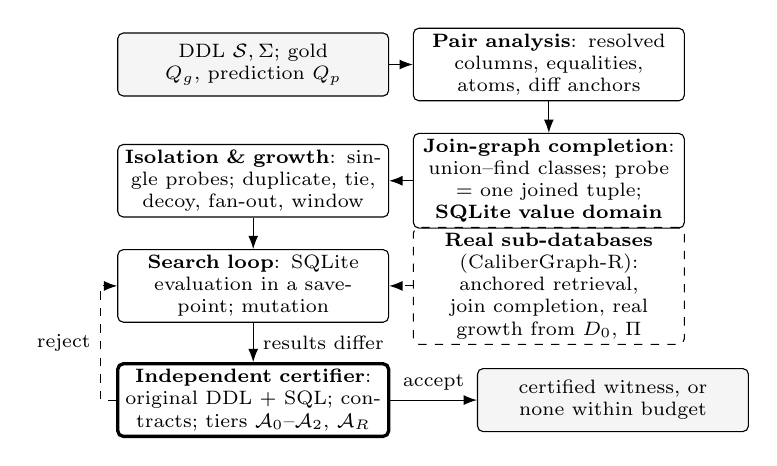
\begin{tikzpicture}[font=\scriptsize,>=Latex,
  box/.style={draw,rounded corners=2pt,align=center,inner sep=2pt,minimum height=8mm,text width=33mm},
  io/.style={box,fill=black!4},
  cert/.style={box,very thick}]
\node[io] (in) at (0,0) {DDL $\mathcal S,\Sigma$; gold $Q_g$, prediction $Q_p$};
\node[box,right=3mm of in] (an) {\textbf{Pair analysis}: resolved columns, equalities, atoms, diff anchors};
\node[box,below=4mm of an] (jg) {\textbf{Join-graph completion}: union--find classes; probe = one joined tuple; \textbf{SQLite value domain}};
\node[box,left=3mm of jg] (iso) {\textbf{Isolation \& growth}: single probes; duplicate, tie, decoy, fan-out, window};
\node[box,below=4mm of iso] (ev) {\textbf{Search loop}: SQLite evaluation in a savepoint; mutation};
\node[box,dashed,right=3mm of ev] (rs) {\textbf{Real sub-databases} (CaliberGraph-R): anchored retrieval, join completion, real growth from $D_0$, $\Pi$};
\node[cert,below=5mm of ev] (ce) {\textbf{Independent certifier}: original DDL + SQL; contracts; tiers $\mathcal A_0$--$\mathcal A_2$, $\mathcal A_R$};
\node[io,right=11mm of ce] (out) {certified witness, or none within budget};
\draw[->] (in)--(an);
\draw[->] (an)--(jg);
\draw[->] (jg)--(iso);
\draw[->] (iso)--(ev);
\draw[->,dashed] (rs)--(ev);
\draw[->] (ev)-- node[right,font=\scriptsize]{results differ} (ce);
\draw[->] (ce)-- node[above,font=\scriptsize]{accept} (out);
\draw[->,dashed] (ce.west) -- ++(-2mm,0) |- node[pos=0.25,left,font=\scriptsize,align=right]{reject} (ev.west);
\end{tikzpicture}
\caption{CaliberGraph pipeline. Candidates built from join-graph probes are evaluated by SQLite; a candidate that separates the queries is returned only if the independent certifier accepts it at the target tier. CaliberGraph-R (dashed) first searches real sub-databases of the benchmark database.}
\label{fig:overview}
\end{figure}


\textbf{Pair analysis and diff anchors.} Both queries are parsed in the SQLite dialect, and column references are resolved to $(T,c)$ through aliases, subqueries and CTEs. For each query $Q$, we collect its tables $\mathrm{tab}(Q)$, its column equalities $E(Q)$, including \texttt{IN}-subquery pairs, and its \emph{atoms} $\mathit{At}(Q)$. An atom is a comparison, \texttt{LIKE}, \texttt{IN}, \texttt{BETWEEN} or \texttt{IS [NOT] NULL} between a column and literals. The column may be wrapped in one function, such as \texttt{strftime}, \texttt{substr}, \texttt{lower}, \texttt{CAST} or $\pm k$. The \emph{anchor atoms} are those whose normal form, with resolved names and a canonical operator, occurs in only one query. The \emph{anchor columns} add every column that is referenced, projected, ordered, grouped or aggregated in only one query. Anchors localize where the queries can disagree.

\textbf{Join-graph completion.} Let $\mathcal T^{*}$ be $\mathrm{tab}(Q_g)\cup\mathrm{tab}(Q_p)$ closed under foreign-key parents. The columns of $\mathcal T^{*}$ are partitioned into classes by the closure of $E(Q_g)\cup E(Q_p)$ and of the foreign keys, computed with union--find. A \emph{probe} assigns one value per class. Its materialization contains one row per referenced table, so that all equated columns agree. A repair step then adds parent rows for dangling foreign keys, fills \texttt{NOT NULL} columns and drops duplicate keys. Key classes receive distinct values in distinct probes.

\textbf{Observation (Reachability).} If a probe makes every atom of the outermost \texttt{WHERE} clause of $Q$ true, its rows form a joined tuple of $Q$ that satisfies the join conditions and filters of $Q$ in the repaired database. Each equality of $E(Q)$ relates columns of one class, which take one value. Repair only adds rows, fills \texttt{NULL}s in \texttt{NOT NULL} columns and drops later duplicates, so the probe's rows are unchanged. Random rows satisfy a join only by chance, which is why fuzzing draws keys from tiny domains. In contrast, probes reach the output by construction whenever their filters hold.

\textbf{SQLite-aware value domain.} Each class receives a pool of values from the atoms on its columns. The pool contains each literal $v$ and, for numeric columns, also $v\pm1$ and $v\pm0.5$, which cover integer division and \texttt{CAST}. For strings, it contains case and padding variants, because \texttt{=} is case-sensitive and \texttt{LIKE} is not. It also contains pre-images under wrapping functions, matching and non-matching \texttt{LIKE} instances, and values strictly between two comparable literals. For example, \texttt{\textquotesingle{}2012-06-15 10:00:00\textquotesingle{}} is a pre-image for \texttt{strftime(\textquotesingle{}\%Y\textquotesingle{},$c$)=\textquotesingle{}2012\textquotesingle{}}. Values are coerced to the declared type, and text of an unobserved shape is replaced by an observed sample.

\textbf{Isolation and controlled growth.} Aggregates, \texttt{DISTINCT}, \texttt{GROUP BY} and \texttt{ORDER BY}\dots\texttt{LIMIT} can \emph{mask} a difference. The search therefore starts from single-probe databases, in which one joined tuple determines the output. It grows them only with operators that target a masking mechanism (Table~\ref{tab:operators}).

\begin{table}[!htbp]
\centering\footnotesize
\caption{Growth operators. Each operator is followed by repair.}\label{tab:operators}
\begin{tabularx}{\linewidth}{@{}l>{\raggedright\arraybackslash}X@{}}
\toprule
Operator & Construction: difference exposed\\
\midrule
duplicate & row copy with fresh keys: \texttt{DISTINCT}, \texttt{COUNT(DISTINCT)}\\
fan-out & $n$ child rows of a join: multiplicity, \texttt{HAVING COUNT}$>n$\\
tie probe & fresh copy tied on ordered columns, both insertion orders: \texttt{LIMIT} tie-breaking\\
window & $\ell{+}o{+}1$ tie probes: rows at \texttt{LIMIT}~$\ell$ \texttt{OFFSET}~$o$ borders\\
literal cover & one probe per equality literal: \texttt{CASE} branches, \texttt{IN} lists\\
decoy & a row that joins nothing: outer joins, anti-joins, \texttt{NOT IN}\\
violating & a probe failing the filters: empty inputs, \texttt{MAX} over no row\\
\bottomrule
\end{tabularx}
\end{table}

\begin{algorithm}[t]
\caption{CaliberGraph. CaliberGraph-R adds line 4.}\label{alg:main}
\footnotesize
\begin{algorithmic}[1]
\Require DDL $(\mathcal S,\Sigma)$, queries $Q_g,Q_p$, tier $\mathcal A$, budget $B$; for $\mathcal A_R$: $D_0$, $\Pi$
\Ensure witness $W\in\mathcal A$ with $\neg\mathcal C_{\mathrm{set}}(Q_g(W),Q_p(W))$, or $\bot$
\State analyze $Q_g,Q_p$: equalities $E$, atoms $\mathit{At}$, anchors
\State union--find column classes over $\mathcal T^{*}$; a value pool per class
\State $\mathit{Pool}\gets\emptyset$
\State \textbf{if} $\mathcal A=\mathcal A_R$: put real sub-databases (anchored retrieval, join completion, real growth) first in the stream
\For{each $D$ in the candidate stream \textbf{while} time $<B$}
  \State $(r_g,r_p)\gets$ run $Q_g,Q_p$ on $D$ in a savepoint
  \If{$\mathrm{set}(r_g)\neq\mathrm{set}(r_p)$ \textbf{and} \Call{Certify}{$D,\mathcal A$}}
    \State \Return $D$ \Comment{re-certified on a fresh connection}
  \EndIf
  \State add $D$ to $\mathit{Pool}$ with weight $=$ number of non-empty results among $r_g,r_p$
\EndFor
\State \Return $\bot$
\Statex \emph{Candidate stream, in order:} single probes for $Q_g$, $Q_p$ and both; two-probe combinations; growth operators (Table~\ref{tab:operators}); boundary and \texttt{NULL} variants of anchor classes; then mutations of parents drawn from $\mathit{Pool}$ by weight, each followed by repair
\end{algorithmic}
\end{algorithm}

\textbf{Search and certification.} The candidate stream (Algorithm~\ref{alg:main}) first enumerates single-probe databases satisfying $Q_g$, $Q_p$ and both. It then enumerates two-probe combinations, the growth structures, and boundary and \texttt{NULL} variants of anchor classes. Finally, it runs a mutation loop until the budget expires. In this loop, parents are weighted by how many queries return rows, and 70\,\% of value changes fall on anchor columns. Each candidate is evaluated in a savepoint of one in-memory SQLite connection, which takes a few hundred microseconds. A candidate on which the results differ is returned only if the certifier accepts it at the target tier, and the certifier is re-run on a fresh connection before reporting. \emph{Soundness} is immediate: a returned $W$ is in $\mathcal A$ and separates the original strings on SQLite. The guarantee is one-sided and relative to the correctness of SQLite and the certifier. CaliberGraph+SC, where SC stands for SpotIt+ constraints, additionally uses the constraints mined by SpotIt+ for value pools and acceptance, so that it has the same knowledge as SpotIt+. No other self-run tool uses them.

\subsection{Data-grounded search for $\mathcal A_R$}\label{sec:realsearch}
CaliberGraph-R changes where candidate rows come from. It reads $\Pi$ and $D_0$, the latter through an indexed read-only copy, and searches \emph{real sub-databases} before synthesis. A sub-database of $D_0$ that is closed under the inclusion dependencies of $\Pi$ satisfies the profile, except for rare rows that violate an approximate cross-key dependency.
\begin{itemize}
\item \emph{Diff-anchored retrieval.} The atoms of each query on table $T$ are translated back to SQL predicates $\varphi_g^T,\varphi_p^T$. Rows with $\varphi_g^T\wedge\neg\varphi_p^T$ or $\varphi_p^T\wedge\neg\varphi_g^T$, on which the filters disagree, are retrieved first. They are followed by rows satisfying both predicates, one, or neither.
\item \emph{Join completion.} Each seed row is completed along the join graph with real related rows, preferably of the same predicate mode. The result is closed under foreign keys, undeclared foreign keys and total participation.
\item \emph{Real growth.} Sub-databases are combined, placing a row that only one query selects next to rows that both select. They are also grown with real rows that tie on an \texttt{ORDER BY} column, the first $k{+}1$ rows of a \texttt{LIMIT}~$k$ window, real \texttt{NULL}s and real duplicates. They are shrunk by single-row deletions, and an entity can be cloned with the rows that reference it.
\item \emph{Constrained synthesis.} If no real sub-database separates the queries, the synthetic search continues from the evaluated sub-databases. It uses pools filtered by $\Pi$, fills untouched columns from real template rows, and applies a repair step that also enforces $\Pi$.
\end{itemize}

\textbf{Example from the development set.} For BIRD question 1020, ``Which player has the highest overall rating?'', $Q_g$ orders \texttt{Player\_Attributes} by \texttt{overall\_rating DESC LIMIT 1}, whereas the Alpha-SQL prediction selects every row equal to the maximum rating. Both return one player on $D_0$. CaliberGraph-R retrieves a real attribute record with rating 84 together with its player, and then adds a \emph{real} record of another player with the same rating. Every row of the resulting four-row database occurs in BIRD. On this database, $Q_g$ returns one player and $Q_p$ returns two. The witness is certified at $\mathcal A_R$ after 28 candidates and 0.22\,s. Whether the prediction or the gold query is right depends on how the question treats ties, which is what attribution judges.

\section{Experimental Setup}\label{sec:setup}

\textbf{Benchmark and systems.} We use the 1,534 questions of the BIRD development set (2024-06-27 revision)~\cite{li2023bird} over eleven SQLite databases with 3--13 tables. Predictions come from the ten systems whose BIRD outputs were released with SpotIt+~\cite{tremante2026spotitplus}: Alpha-SQL~\cite{li2025alphasql}, CHESS~\cite{talaei2024chess}, CSC-SQL-7B/32B~\cite{sheng2025cscsql}, two GenaSQL submissions~\cite{donder2025genasql}, GSR (an anonymous entry listed in~\cite{tremante2026spotitplus}), OmniSQL-32B~\cite{li2025omnisql}, RSL-SQL~\cite{cao2024rslsql} and SLM-SQL~\cite{sheng2025slmsql}, covering multi-agent pipelines, fine-tuned 7B--32B models and self-consistency. BIRD is the only Text-to-SQL benchmark for which verifier outputs on many systems have been released, which lets us compare all tool families on identical inputs, and its databases are large real instances (3.9\,M rows), which tier $\mathcal A_R$ needs. We recomputed the released EX labels on the official databases; they agree on 15,339 of 15,340 pairs (the exception depends on the current date). The held-out schemas are \texttt{formula\_1}, \texttt{superhero} and \texttt{toxicology}. Development has 349 questions and test 1,174, i.e.\ 11,740 test (system, question) pairs: \V{nExc} EX-correct (6,456 distinct predictions) and 3,745 EX-incorrect.

\textbf{Baselines.} They cover the main families of judging a prediction beyond EX, each with a strong public representative for SQLite and BIRD:
\begin{itemize}
\item \emph{Random fuzzing} in the style of test-suite accuracy~\cite{zhong2020testsuite}: 1--5 random rows per referenced table with values from both queries' literals, observed value samples, type-faithful values and \texttt{NULL}; keys from a three-value domain so that joins occur; foreign and primary keys repaired. It shares CaliberGraph's value coercion and certifier, but no join graph, anchors or isolation.
\item \emph{ParSEval}~\cite{chen2025parseval} (commit \texttt{88cfe245}, Z3 4.16.0), coverage-driven symbolic generation. ParSEval-L1 keeps its generator but accepts only certified databases, restarts with new seeds until the budget is spent, and receives the same observed format samples; its unmodified \texttt{disprove} routine is reported as ParSEval (official). ParSEval's solver exceeded the budget and was stopped on 732 of the 6,456 distinct pairs.
\item \emph{SpotIt}~\cite{klopfenstein2026spotit} and \emph{SpotIt+}~\cite{tremante2026spotitplus}, bounded verification without and with LLM-validated mined constraints (released outputs; SpotIt also re-run under our budget, Section~\ref{sec:main}).
\end{itemize}
\emph{Excluded tools.} Provers such as SQLSolver~\cite{ding2023sqlsolver} and QED~\cite{wang2024qed} establish equivalence and return no counterexample database; VeriEQL~\cite{he2024verieql} is represented by SpotIt, which builds on it and reports BIRD results; XData~\cite{chandra2015xdata} and EvoSQL~\cite{castelein2018evosql} generate tests for one query or a mutant space rather than for a given pair. LLM judges~\cite{kim2025flex} produce no checkable evidence.

For the second freeze, \emph{random fuzzing-R} draws 1--5 real rows per referenced table from $D_0$ or template rows, re-draws referenced columns from literals, observed values and \texttt{NULL}, and closes the result under foreign keys and total participation with real rows; \emph{ParSEval-R} gives ParSEval a value provider that returns observed values first; because its solver still introduces unobserved values, it is a weak baseline at this tier, and we do not claim a fair comparison with symbolic generation at $\mathcal A_R$. Both receive the same read access to $D_0$, profile, repair and certifier-in-the-loop acceptance at $\mathcal A_R$ as CaliberGraph-R.

\textbf{Budgets and platform.} All self-run tools get 5\,s wall-clock per distinct pair on one core (two workers on a 2-core VM with 7\,GB of memory); a 10\,s budget is evaluated on a random subsample of \V{nSub} distinct pairs, which is also used for ablations. ParSEval-R certified none of 600 development pairs and was therefore run on this subsample only (decided before the second test run). CaliberGraph is implemented in Python 3.13 with SQLGlot and SQLite 3.45. Code, splits, raw outputs, witnesses, certifier reports, annotations and the pre-registrations are in the artifact repository.

\section{Results}\label{sec:results}

All numbers are computed on the test questions by scripts from the saved outputs; counts are over (system, question) pairs unless stated otherwise. Table~\ref{tab:overview} summarises every tool at every tier and Table~\ref{tab:hypotheses} the pre-registered hypotheses; analyses that were not pre-registered are marked \emph{post hoc}.

% Overview table (journal version, portrait): (a) certified pairs and recall, (b) attribution. Numbers are macros.
\begin{table}[!htbp]
\centering\small
\caption{Overview on the test pairs. \emph{Certified}: EX-correct pairs ($n=\V{nExc}$) with a witness that our certifier accepts at each tier (re-certified released counterexamples for SpotIt/SpotIt+; SpotIt (re-run): our local re-run under the common budget); \emph{Claimed}: pairs the released results classify as non-equivalent. \emph{Recall}: share of known positives ($n=\V{nExi}$) with a witness. \emph{Attribution}: random sample of 100 witnesses per tool at the tier given in parentheses; \emph{Est.\ meaningful}: certified count $\times$ meaningful share (95\,\% CI). --: not applicable or not sampled.}\label{tab:overview}
\setlength{\tabcolsep}{4pt}
\begin{tabular}{@{}l r rrrrr rr@{}}
\toprule
& & \multicolumn{5}{c}{Certified EX-correct pairs} & \multicolumn{2}{c}{Recall (\%)}\\
\cmidrule(lr){3-7}\cmidrule(l){8-9}
Tool & Claimed & $\mathcal A_0$ & $\mathcal A_{1f}$ & $\mathcal A_2$ & $\mathcal A_{Rq}$ & $\mathcal A_R$ & $\mathcal A_{1f}$ & $\mathcal A_R$\\
\midrule
SpotIt & \V{nSIClaims} & \V{nSILzero} & \V{nSILonef} & \V{nSILtwo} & \V{nSIAtRq} & \V{nSIAtR} & \V{rSI}$^{*}$ & --\\
SpotIt (re-run) & \V{srClaims} & \V{srLzero} & \V{srLonef} & -- & \V{srRq} & \V{srR} & -- & --\\
SpotIt+ & \V{nSIPClaims} & \V{nSIPLzero} & \V{nSIPLonef} & \V{nSIPLtwo} & \V{nSIPAtRq} & \V{nSIPAtR} & -- & --\\
ParSEval (official) & -- & \V{nPVOLzero} & \V{nPVOLonef} & \V{nPVOLtwo} & -- & -- & -- & --\\
ParSEval-L1 & -- & \V{nPVLzero} & \V{nPVLonef} & \V{nPVLtwo} & \V{nPVAtRq} & \V{nPVAtR} & \V{rPVLonef} & --\\
Random fuzzing & -- & \V{nFZLzero} & \V{nFZLonef} & \V{nFZLtwo} & \V{nFZAtRq} & \V{nFZAtR} & \V{rFZLonef} & --\\
CaliberGraph & -- & \V{nCGLzero} & \V{nCGLonef} & \V{nCGLtwo} & \V{nCGAtRq} & \V{nCGAtR} & \V{rCGLonef} & --\\
CaliberGraph+SC & -- & \V{nCGSCLzero} & \V{nCGSCLonef} & \V{nCGSCLtwo} & \V{nCGSCAtRq} & \V{nCGSCAtR} & -- & --\\
\midrule
Random fuzzing-R & -- & \V{nFZRAtLonef} & \V{nFZRAtLonef} & \V{nFZRAtLtwo} & \V{nFZRAtRq} & \V{nFZRAtR} & \V{rFZRAtLonef} & \V{rFZRAtR}\\
CaliberGraph-R & -- & \V{nCGRAtLonef} & \V{nCGRAtLonef} & \V{nCGRAtLtwo} & \V{nCGRAtRq} & \V{nCGRAtR} & \V{rCGRAtLonef} & \V{rCGRAtR}\\
\bottomrule
\end{tabular}

\medskip
\begin{tabular}{@{}l l r l@{}}
\toprule
Tool & Implausible \% (tier) & Meaningful \% & Est.\ meaningful [95\,\% CI]\\
\midrule
SpotIt & \V{pSIImpl} ($\mathcal A_0$) & \V{pSIMeaningful} & \V{estSIMeaningful} \V{estSIMeaningfulCI}\\
SpotIt+ & \V{pSIPImpl} ($\mathcal A_0$) & \V{pSIPMeaningful} & \V{estSIPMeaningful} \V{estSIPMeaningfulCI}\\
ParSEval-L1 & \V{pPVImpl} ($\mathcal A_{1f}$) & \V{pPVMeaningful} & \V{estPVMeaningful} \V{estPVMeaningfulCI}\\
Random fuzzing & \V{pFZImpl} ($\mathcal A_{1f}$) & \V{pFZMeaningful} & \V{estFZMeaningful} \V{estFZMeaningfulCI}\\
CaliberGraph & \V{pCGImpl} ($\mathcal A_{1f}$) & \V{pCGMeaningful} & \V{estCGMeaningful} \V{estCGMeaningfulCI}\\
\midrule
Random fuzzing-R & \V{pFZRImpl} ($\mathcal A_R$) & \V{pFZRMeaningful} & \V{estFZRMeaningful} \V{estFZRMeaningfulCI}\\
CaliberGraph-R & \V{pCGRImpl} ($\mathcal A_R$) & \V{pCGRMeaningful} & \V{estCGRMeaningful} \V{estCGRMeaningfulCI}\\
\bottomrule
\end{tabular}

\smallskip
\parbox{\linewidth}{\footnotesize $^{*}$Share of known positives SpotIt claims non-equivalent (uncertified). ParSEval-R certified none of the \V{nSubR} subsample pairs (Section~\ref{sec:setup}) and is omitted. The second-stage tools search at $\mathcal A_R$ only; their $\mathcal A_0$--$\mathcal A_2$ entries re-evaluate the same witnesses ($\mathcal A_R\subseteq\mathcal A_{1f}\subseteq\mathcal A_0$).}
\end{table}

% ICDE: pre-registered hypotheses and outcomes; numbers are macros from numbers.tex / numbers_icde.tex
\begin{table}[!htbp]
\centering\scriptsize
\caption{Pre-registered hypotheses and outcomes on the test pairs. $\Delta$ is the difference in pairs, or in estimated meaningful witnesses for H6, with a 95\,\% CI from a bootstrap over questions. For H1--H5, $p$ is from an exact McNemar test, Holm-adjusted within H1--H3 and, post hoc, across the four H4 components. H6 uses a one-sided bootstrap, parametric as pre-registered; a bootstrap over questions gives CI \V{hSixClusterCI} and $p$ \V{hSixClusterP}. H7 uses a one-sided bootstrap over questions. Stage~3 uses one-sided tests (R3-4 is two-sided), Holm-adjusted over its eight tests. C1 and C2 share a row; C2 gives \V{arcApct} vs.\ \V{arcANpct}\,\%, with adjusted $p$ \V{holmCTwo}. R2 and R3 were pre-registered separately and are not adjusted. SP1--SP2 were pre-registered separately and are Holm-adjusted together. $\kappa_2$ is Cohen's $\kappa$ (Fleiss' for R3-1) on implausible vs.\ other.}\label{tab:hypotheses}
\setlength{\tabcolsep}{3pt}
\begin{tabular}{@{}l p{60mm} l l c@{}}
\toprule
& Comparison & $\Delta$ [95\,\% CI] & $p$ & Result\\
\midrule
H1 & CG at $\mathcal A_{1f}$ vs SpotIt claims & \V{hOneDiff} \V{hOneCI} & $<10^{-10}$ & yes\\
H2 & CG+SC at $\mathcal A_2$ vs SpotIt+ claims & \V{hTwoDiff} \V{hTwoCI} & $<10^{-10}$ & yes\\
H3 & recall: CG vs ParSEval-L1 / SpotIt & \V{rCGLonef} vs \V{rPVLonef} / \V{rSI}\,\% & $<10^{-10}$ & yes\\
H4 & each component's removal lowers the count & join graph only ($-$11) & 0.004 & no\\
H5 & CG-R vs fuzzing-R at $\mathcal A_R$ & \V{tCGRvsFZRRDiff} \V{tCGRvsFZRRCI} & $<10^{-10}$ & yes\\
   & CG-R vs ParSEval-R (subsample) & \V{ablRFull} vs \V{ablRPV} & $<10^{-10}$ & \\
H6 & est.\ meaningful, CG-R vs fuzzing-R & \V{hSixDiff} \V{hSixCI} & \V{hSixP} & weak\\
H7 & implausible share, CG-R vs CG & \V{pCGRImpl} vs \V{pCGImpl}\,\% & $<10^{-4}$ & yes\\
\midrule
\multicolumn{5}{@{}l}{\emph{Stage 3 (attribution validity and replication)}}\\
A1 & humans without $D_0$ agree with each other & $\kappa_2$ \V{hvKappaHHbin} & & no\\
A2--3 & \quad with AI; tier gap & $\kappa_2$ \V{hvKappaHAbinMin}--\V{hvKappaHAbinMax}; \V{hvImpConsOne}/\V{hvConsOne} vs \V{hvImpConsTwo}/\V{hvConsTwo} & \V{holmAThree} & no\\
R2 & humans with facts of $D_0$: tier gap & \V{hvTwoImpConsOne}/\V{hvTwoConsOne} vs \V{hvTwoImpConsTwo}/\V{hvTwoConsTwo} & \V{hvTwoP} & yes\\
   & \quad agree with each other / with AI & $\kappa_2$ \V{hvTwoKappaBin} / \V{hvTwoKappaAIbinMax} & & yes / no\\
B & second model vs AI; tier gap & $\kappa_2$ \V{cmKappaBin}; \V{cmImpOne} vs \V{cmImpTwo}\,\% & \V{holmBTwo} & yes\\
C & our issues vs Arcwise-Plat corrections & \V{arcGpct} vs \V{arcNpct}\,\% (gold) & \V{holmCOne} & no\\
S1 & Spider: CG-R vs fuzzing-R at $\mathcal A_R$ & \V{spRCG} vs \V{spRFZ} & \V{holmSOne} & no\\
S2 & Spider: implausible, CG-R vs CG & \V{spImpCGR} vs \V{spImpCG} of 60 & \V{holmSTwo} & no\\
S3 & Spider: est.\ meaningful, CG-R vs fuzzing-R & \V{spEstCGR} vs \V{spEstFZR} & \V{holmSThree} & rev.\\
E1 & 13 new BIRD systems: CG-R vs fuzzing-R & \V{mdDiff} [\V{mdLo}, \V{mdHi}] & \V{holmEOne} & yes\\
R3-1 & three humans agree (Fleiss) & $\kappa_2$ \V{hvThreeFleissBin} & & no\\
R3-2 & \quad majority vs AI & $\kappa_2$ \V{hvThreeKappaAIbin} & & no\\
R3-3 & \quad majority: tier gap & \V{hvThreeImpOne}/\V{hvThreeMajOne} vs \V{hvThreeImpTwo}/\V{hvThreeMajTwo} & \V{hvThreePThree} & yes\\
R3-4 & \quad pred.\ errors at $\mathcal A_R$, majority vs AI & \V{hvThreeErrHumTwo} vs \V{hvThreeErrAITwo} of \V{hvThreeMajTwo} & \V{hvThreePFour} & yes\\
SP1 & CG vs SpotIt re-run, $\mathcal A_{1f}$ & \V{srOneDiff} \V{srOneCI} & $<10^{-10}$ & yes\\
SP2 & \quad at $\mathcal A_0$ & \V{srTwoDiff} \V{srTwoCI} & $<10^{-10}$ & yes\\
\bottomrule
\end{tabular}
\end{table}


\subsection{RQ1: Certified witnesses at schema-derived tiers}\label{sec:main}
At the primary tier $\mathcal A_{1f}$, CaliberGraph certifies \V{nCGLonef} of the \V{nExc} EX-correct pairs (\V{pCGLonef}\,\%). Re-run locally under the same five-second budget (Stage~3, pre-registered), the original SpotIt claims \V{srClaims} pairs, and \V{srLzero} of its counterexamples are certified at $\mathcal A_0$ and \V{srLonef} at $\mathcal A_{1f}$; CaliberGraph certifies \V{srOneDiffAbs} more pairs at $\mathcal A_{1f}$ (95\,\% CI \V{srOneCI}; H-SP1) and \V{srTwoDiffAbs} more at $\mathcal A_0$ (CI \V{srTwoCI}; H-SP2), and only \V{srTwoSIonly} pairs have an $\mathcal A_0$ witness from SpotIt alone. $\mathcal A_0$ is the fairer comparison: SpotIt receives no format samples, stops at its first validated rather than first certified counterexample, and models MySQL semantics on upper-cased queries, so part of its loss reflects the mismatch with SQLite rather than its search. The re-run reproduces \V{srRefoundPct}\,\% of the released claims (distinct pairs), so the short budget costs about \V{srLossPct}\,\%; \V{srKilledPct}\,\% of distinct pairs exhaust it, \V{srErr} end in a solver error, the median time to a counterexample is \V{srMedCE}\,s, and restoring the literals' case (diagnostic) certifies fewer pairs (\V{srRecased} at $\mathcal A_0$). Against SpotIt's released claims, which are counted without certification and took up to about 20 minutes per pair, CaliberGraph certifies \V{hOneDiff} more (CI \V{hOneCI}; H1). Under identical budgets, acceptance tests and format knowledge, ParSEval-L1 certifies \V{nPVLonef} pairs and random fuzzing \V{nFZLonef}; only \V{vsPVBOnly} and \V{vsFZBOnly} of their pairs lack a CaliberGraph witness. CaliberGraph's lead is specific to these tiers: at $\mathcal A_2$, whose LLM-validated constraints none of the three tools uses, random fuzzing certifies more pairs (\V{nFZLtwo} vs \V{nCGLtwo}); given those constraints, CaliberGraph+SC certifies \V{nCGSCLtwo} pairs against \V{nSIPClaims} claimed by SpotIt+ (H2). With the official full-column format profiles (a pre-registered sensitivity check), CaliberGraph keeps \V{nCGOonef} pairs, ParSEval-L1 \V{nPVOonef}, fuzzing \V{nFZOonef}, and SpotIt, SpotIt+ and CaliberGraph+SC none.

Released verifier counterexamples lose many pairs on re-certification: of SpotIt's \V{nSIClaims} claims, \V{nSILzero} counterexamples still separate the original queries on SQLite and satisfy the DDL, and \V{nSILonef} are also format-faithful (SpotIt+: \V{nSIPLzero} and \V{nSIPLonef} of \V{nSIPClaims}). On development data, the loss at $\mathcal A_0$ was traced mainly to preprocessing (upper-cased literals, unmodelled \texttt{NOT NULL} and \texttt{UNIQUE} constraints) rather than to wrong verdicts; the further loss comes from implausible value formats. Multiset equality leaves every count unchanged (Table~\ref{tab:contracts} in the appendix), and the lenient $\mathcal C_{\mathrm{len}}$ keeps \V{nCGLonefLenient} of CaliberGraph's \V{nCGLonef} pairs.


\subsection{RQ2: What do the witnesses show? (post hoc)}\label{sec:attrresults}
% generated by src_s3/s3a_table.py
\begin{table}[!htbp]
\centering\scriptsize
\caption{Human estimates next to the AI estimates (pre-registered reporting rule): verdicts on the same blind items, per round and stage (stage 1: schema-tier witnesses; stage 2: $\mathcal A_R$). Humans: rounds 1--2, items on which both annotators agree (Dis.: they disagree); round 3, the label of at least two of three annotators (Dis.: no majority). Round 1 showed only the witness, rounds 2--3 also facts of $D_0$. AI counts are over all items (R3-4 in Table~\ref{tab:hypotheses} compares the 64 stage-2 items with a majority).}\label{tab:humanai}
\setlength{\tabcolsep}{3pt}
\begin{tabular}{@{}llrrrrrrr@{}}
\toprule
Round & Stage, judge & $n$ & Pred.\ err. & Both & Gold err. & Ambig. & Implaus. & Dis.\\
\midrule
1 & 1, AI & 30 & 0 & 0 & 8 & 8 & 14 & \\
 & 1, humans & 30 & 8 & 0 & 18 & 1 & 0 & 3\\
\addlinespace[1pt]
 & 2, AI & 30 & 4 & 0 & 7 & 12 & 7 & \\
 & 2, humans & 30 & 11 & 1 & 11 & 1 & 0 & 6\\
\midrule
2 & 1, AI & 30 & 3 & 1 & 4 & 6 & 16 & \\
 & 1, humans & 30 & 4 & 0 & 1 & 0 & 20 & 5\\
\addlinespace[1pt]
 & 2, AI & 30 & 3 & 1 & 3 & 12 & 11 & \\
 & 2, humans & 30 & 14 & 0 & 2 & 1 & 9 & 4\\
\midrule
3 & 1, AI & 75 & 9 & 1 & 10 & 13 & 42 & \\
 & 1, humans & 75 & 11 & 0 & 24 & 7 & 10 & 23\\
\addlinespace[1pt]
 & 2, AI & 75 & 11 & 0 & 18 & 31 & 15 & \\
 & 2, humans & 75 & 18 & 0 & 28 & 18 & 0 & 11\\
\bottomrule
\end{tabular}
\end{table}



\begin{figure}[!htbp]
\centering
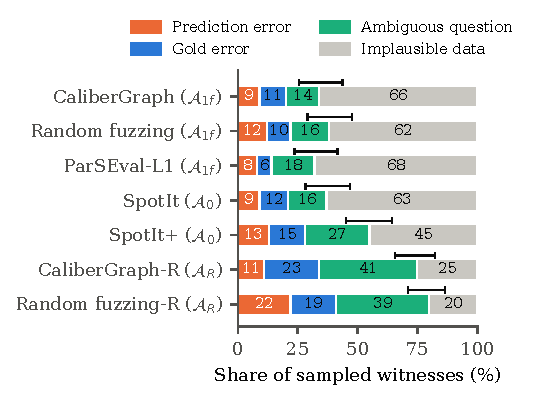
\includegraphics[width=0.8\linewidth]{figs/attribution.pdf}
\caption{Attribution of random samples of 100 witnesses per tool (LLM annotation: two tool-blind passes, adjudicated). Upper five bars: first-stage tools at $\mathcal A_{1f}$ (SpotIt and SpotIt+ at $\mathcal A_0$); lower two: second-stage tools at $\mathcal A_R$.}\label{fig:attribution}
\end{figure}

The two annotation passes agree on \V{attrAgree}\,\% of the \V{attrN} first-stage witnesses ($\kappa=\V{attrKappa}$); \V{attrAdj} disagreements were adjudicated. For every tool, \V{attrImplMin}--\V{attrImplMax}\,\% of the sampled witnesses separate the queries only on implausible data, and only \V{attrErrMin}--\V{attrErrMax}\,\% expose an error of the prediction (Fig.~\ref{fig:attribution}; CaliberGraph: \V{pCGImpl}\,\% implausible, CI over questions \V{pCGImplClusterCI}). The decisive implausible facts are of few kinds: \texttt{NULL} in a column that is never \texttt{NULL} in BIRD; duplicates of what is unique in reality (a badge awarded twice, two races of one Grand Prix in a season); values that do not occur (a negative round, an atom identifier of the wrong pattern); and inconsistent records (a school whose county differs between two tables, a bond stored in one direction, an account without owner). Weighted by certified counts, CaliberGraph yields an estimated \V{estCGMeaningful} meaningful witnesses \V{estCGMeaningfulCI} and random fuzzing \V{estFZMeaningful} \V{estFZMeaningfulCI}: CaliberGraph's lead of \V{vsFZDiff} certified pairs over fuzzing does \emph{not} carry over to meaningful witnesses, and the estimated prediction errors its witnesses expose (\V{estCGErr}) are not more than fuzzing's (\V{estFZErr}). Of the \V{nSIClaims} pairs SpotIt claims to be non-equivalent, \V{nSILzero} can be re-certified, and an estimated \V{estSIErr} of these expose a prediction error. Since attribution judges the returned witness, not the pair, these are lower bounds on errors among certified pairs.

\textbf{Is the attribution valid? (Stage 3, pre-registered.)} Human annotators labelled random samples of witnesses, half from each stage, independently and blind to tool, tier and AI verdict, in three rounds (Table~\ref{tab:humanai}; $\kappa_2$: Cohen's or, for three annotators, Fleiss' $\kappa$ on implausible vs.\ other). In round~1 two annotators saw only the witness and the queries: they agreed with each other on the five labels ($\kappa=\V{hvKappaHH}$) but not with the AI ($\kappa=\V{hvKappaHAmin}$--\V{hvKappaHAmax}), and chose \emph{implausible data} only \V{hvImpHOne} and \V{hvImpHTwo} times among the 30 first-stage witnesses, where the AI chose it \V{hvImpAIOne} times. Many of their reasons describe the anomaly the AI cites --- e.g., a lookup row \texttt{(3,'Bad')} where BIRD stores \texttt{(3,'Neutral')} --- but resolve it as an error of one query \emph{on the witness}. In round~2 every item also showed mechanically generated facts about $D_0$ (\texttt{NULL} counts, uniqueness and frequencies of the witness values of each referenced column), and the instructions asked first whether the difference could arise on real data (round~3 dropped this order). The same annotators then agreed on implausibility ($\kappa_2=\V{hvTwoKappaBin}$, CI \V{hvTwoKappaBinLo}--\V{hvTwoKappaBinHi}) and reproduced the gap between the tiers (\V{hvTwoImpConsOne}/\V{hvTwoConsOne} vs.\ \V{hvTwoImpConsTwo}/\V{hvTwoConsTwo} agreed witnesses; $p=\V{hvTwoP}$), but agreed with the AI only moderately ($\kappa_2=\V{hvTwoKappaAIbinMax}$) and called many more witnesses prediction errors and almost none ambiguous. Round~3, pre-registered after an independent pre-submission review asked for more annotators, gave three unpaid volunteers, data analysts in e-commerce and social media, \V{hvThreeN} new witnesses with the same facts and the AI annotator's label definitions verbatim. They agreed with each other barely above chance (Fleiss' $\kappa=\V{hvThreeFleissFive}$, $\kappa_2=\V{hvThreeFleissBin}$, CI \V{hvThreeFleissBinLo}--\V{hvThreeFleissBinHi}), choosing \emph{implausible data} \V{hvThreeImpA}, \V{hvThreeImpB} and \V{hvThreeImpC} times (AI: \V{hvThreeImpAI}); \V{hvThreeNoMaj} items have no majority label. The majority agreed with the AI with $\kappa_2=\V{hvThreeKappaAIbin}$, called \V{hvThreeImpOne}/\V{hvThreeMajOne} first-stage and \V{hvThreeImpTwo}/\V{hvThreeMajTwo} second-stage witnesses implausible ($p=\V{hvThreePThree}$), and saw more prediction errors than the AI at $\mathcal A_R$ (\V{hvThreeErrHumTwo} vs.\ \V{hvThreeErrAITwo}; $p=\V{hvThreePFour}$). We report the round as received, although its process record is imperfect: the start and finish times recorded on the sheets are partly impossible (one finish lies after the return, one start before the sheets existed) and differ from the authors' later account that all three annotated by hand from 11:00 to 14:00 on the day of distribution, i.e., about 1.2 minutes per item against an estimated three; one annotator gave 24 distinct, mostly generic reasons for 150 items; and one sheet passed through an editor that removed tag-like values from two items and turned a URL in a third into a link. All three reported working without AI tools. Without the annotator with generic reasons (post hoc), the other two agree on implausibility with $\kappa_2=\V{hvThreeKappaBCbin}$. By the pre-stated rules, neither the five-label attribution nor the implausibility judgement is reliably reproducible by humans; the AI shares below are one annotator's operational judgement. A second model (Claude Sonnet~5.5) with the AI annotator's prompt and data access agreed with it ($\kappa=\V{cmKappaBin}$ on \V{cmN} witnesses) and reproduced the stage gap (\V{cmImpOne} vs.\ \V{cmImpTwo} of 100).

\textbf{An annotator-free test (post hoc).} We repaired each first-stage witness locally, replacing the cells that violate the data profile $\Pi$ (Section~\ref{sec:profile}) by real values in 20 random repairs, and re-ran both queries. The difference vanished on every repair for \V{xVan} of \V{xN} witnesses (\V{xVanPct}\,\%) and survived on some for \V{xSurv}; it vanished for \V{xImpVanPct}\,\% of the witnesses the AI called implausible, but also for \V{xOthVanPct}\,\% of the others, and it vanished for \V{xHumVan} of the \V{xHumRep} repaired first-stage witnesses that both round-2 annotators called implausible. Yet for \V{xVanPairARpct}\,\% of the witnesses whose difference vanished (and \V{xPairARpct}\,\% of all), CaliberGraph-R or fuzzing-R found an $\mathcal A_R$ witness for the same pair: the two queries do differ on realistic data, but the first-stage witness does not show it. Without the facts, the round-1 annotators judged the \emph{pair} (which query answers the question); the AI, the round-2 annotators and the repair test judge the \emph{witness} (whether this database is evidence of that difference). The three are not independent of our definition: the facts shown in round~2 and the cells the repair replaces both come from $D_0$ and its profile, so they test the consistency of an operational notion of realism, not realism itself.


\subsection{RQ3: Data-grounded witnesses}\label{sec:rresults}

\begin{table}[!htbp]
\centering\footnotesize
\caption{The data profile $\Pi$ mined from the eleven BIRD databases (75 tables, 3.9\,M rows; 258\,s on one core) and the share of first-stage $\mathcal A_{1f}$ witnesses (distinct EX-correct pairs) that violate each constraint class on the columns either query references (post hoc). CG: CaliberGraph; PSE: ParSEval-L1.}\label{tab:profile}
\setlength{\tabcolsep}{2pt}\scriptsize
\Tab{profile_icde}
\end{table}

None of CaliberGraph's \V{nCGLonef} first-stage witnesses satisfies the full data profile, and \V{nCGAtRq} satisfy it on the referenced columns. Column-level mined constraints do not close the gap: CaliberGraph+SC certifies \V{nCGSCLtwo} pairs at $\mathcal A_2$ but only \V{nCGSCAtR} at $\mathcal A_R$, none of SpotIt+'s \V{nSIPLtwo} $\mathcal A_2$ counterexamples reaches $\mathcal A_R$, and \V{pSIPImpl}\,\% of SpotIt+'s sampled witnesses are implausible. CaliberGraph-R certifies \V{nCGRAtR} EX-correct pairs (\V{pCGRAtR}\,\%) at $\mathcal A_R$, against \V{nFZRAtR} for random fuzzing-R with the same data access, repair and acceptance (difference \V{tCGRvsFZRRDiff}, CI \V{tCGRvsFZRRCI}); ParSEval-R certifies \V{ablRPV} of the \V{nSubR} subsample pairs, on which CaliberGraph-R certifies \V{ablRFull}. H5 is supported, and the lead holds on the schemas held out in the first stage, which informed the tier's design (\V{rateCGRHeld} vs \V{rateFZRHeld}\,\% of EX-correct pairs), as on the others (\V{rateCGROther} vs \V{rateFZROther}\,\%).

\textbf{Why schema-tier witnesses fail the profile (post hoc).} On the columns the queries reference (Table~\ref{tab:profile}), 72--86\,\% of the first-stage witnesses use a value outside the column's observed domain (an unseen category, shape or range), 30--70\,\% put a \texttt{NULL} into one of the 420 columns that are never \texttt{NULL} in BIRD, and 21--56\,\% break a value dependency (e.g., a county code paired with another county's name); half of ParSEval's minimal instances also duplicate a unique column combination. Every constraint class is violated by some tool's witnesses. Certified counts are insensitive to the categorical thresholds of the profile: re-certifying the stored witnesses with halved or doubled thresholds changes CaliberGraph-R's \V{thrCGRFrozen} distinct certified pairs to \V{thrCGRLooser} (halved) and \V{thrCGRStricter} (doubled) and fuzzing-R's \V{thrFZRFrozen} to \V{thrFZRLooser} and \V{thrFZRStricter}, and admits none of CaliberGraph's first-stage witnesses. The check varies only the categorical thresholds; the never-\texttt{NULL} rule and the dependency classes were not varied.

\textbf{What the tier changes.} \V{pCGRImpl}\,\% of CaliberGraph-R's sampled witnesses rely on implausible data (CI over questions \V{pCGRImplClusterCI}), against \V{pCGImpl}\,\% of CaliberGraph's $\mathcal A_{1f}$ witnesses (H7; one-sided $p=\V{hSevenP}$, and $p\V{hSevenClusterP}$ over questions; pass agreement \V{attrRAgree}\,\%, $\kappa=\V{attrRKappa}$). The drop holds on the first-stage held-out schemas (\V{implCGRHeld} vs \V{implCGHeld}) and on the others (\V{implCGROther} vs \V{implCGOther}); fifty first-stage witnesses re-annotated in the same batch received the same verdict in \V{calibSame} cases, so it is not annotator drift. The rise in the meaningful share is due to the tier, not to the search: random fuzzing-R reaches \V{pFZRMeaningful}\,\%. CaliberGraph-R yields an estimated \V{estCGRMeaningful} meaningful witnesses against \V{estFZRMeaningful} for fuzzing-R; the difference (\V{hSixDiff}) was significant under the pre-registered parametric bootstrap (CI \V{hSixCI}, $p=\V{hSixP}$) but not robustly so under a bootstrap over questions (CI \V{hSixClusterCI}, one-sided $p=\V{hSixClusterP}$), so we regard H6 as only weakly supported. Post hoc, fuzzing-R's witnesses show a prediction error more often (estimated \V{estFZRErr} against \V{estCGRErr}); as its certified pairs are almost a subset of CaliberGraph-R's (\V{tCGRvsFZRRBOnly} exceptions), the difference lies in \emph{which} witness is returned for a pair.

\textbf{A limitation of the tier.} A sub-database may omit the entity a question names, so that one query returns no row and the other a row of \texttt{NULL}s (\V{nEmptyNullCGR} of CaliberGraph-R's and \V{nEmptyNullFZR} of fuzzing-R's 100 sampled witnesses, all but one of which the attribution counts as meaningful); under $\mathcal C_{\mathrm{len}}$, which equates the two, they certify \V{nCGRAtRClen} and \V{nFZRAtRClen} pairs.

\textbf{A meaningful data-grounded witness.} For ``How many cards available in paper have a positive starting maximum hand size?'' the evidence defines availability as \texttt{LIKE '\%paper\%'}, but the gold query tests \texttt{availability = 'paper'}; CaliberGraph-R returns three real cards, one with the observed value \texttt{'arena,mtgo,paper'}, on which the gold query counts one card and the prediction two --- a gold query that contradicts its own evidence.

\textbf{Recall on known positives.} CaliberGraph finds an $\mathcal A_{1f}$ witness for \V{rCGLonef}\,\% of the \V{nExi} known positives, against \V{rPVLonef}\,\% for ParSEval-L1, \V{rFZLonef}\,\% for fuzzing and \V{rSI}\,\% claimed by SpotIt (H3). At $\mathcal A_R$ the figure is a sanity check rather than an estimate: $D_0$ itself separates every known positive and satisfies its profile up to the approximate cross-key rules, and CaliberGraph-R finds a witness for \V{rCGRAtR}\,\% (fuzzing-R \V{rFZRAtR}\,\%). No recall estimate exists for EX-correct pairs, on which a missed difference is invisible.


\subsection{RQ4: Effect on accuracy and rankings}\label{sec:rankings}

\begin{table}[!htbp]
\centering\footnotesize
\caption{Per-system effect on the 1,174 test questions. Count-based: share of EX-correct predictions with a CaliberGraph $\mathcal A_{1f}$ witness, and EX after removing all of them (EX$'$). Error-weighted: certified share $\times$ attributed prediction-error rate (\V{errShareCG}\,\% at $\mathcal A_{1f}$, \V{errShareCGR}\,\% at $\mathcal A_R$), in points of EX; a lower bound (post hoc).}\label{tab:systems}
\setlength{\tabcolsep}{3pt}
\Tab{systems_icde}
\end{table}

Counting every $\mathcal A_{1f}$ witness as an error, \V{fpShareMin}--\V{fpShareMax}\,\% of each system's EX-correct predictions are removed, EX drops by \V{exDropMin}--\V{exDropMax} points and six to eight of the ten systems change rank, depending on how two exact EX ties are broken (Kendall's $\tau_b=\V{kendallTau}$; Table~\ref{tab:systems}); SpotIt's claims imply \V{ptsCountSpotItMin}--\V{ptsCountSpotItMax} points. RQ2 shows that most of these witnesses are not errors. Weighting each system's certified share (CaliberGraph at $\mathcal A_{1f}$, CaliberGraph-R at $\mathcal A_R$) by that tool's attributed prediction-error rate gives \V{ptsErrOnefMin}--\V{ptsErrOnefMax} points per system at $\mathcal A_{1f}$ and \V{ptsErrRMin}--\V{ptsErrRMax} at $\mathcal A_R$ (post hoc), with rankings unchanged except within the two exact ties ($\tau_b=\V{tauErrOnef}$ at both tiers, by construction, as one error rate is applied per tier). The estimates are lower bounds if the labels are unbiased, since a pair whose returned witness is implausible may still be an error (CaliberGraph-R's AI error rate: \V{errShareCGR}\,\%, interval over questions about 5--18\,\%). They also depend on who attributes. With the round-3 human majority's error rates (pre-registered, but of limited reliability given H-R3-1; \V{humThreeErrPctOnef}\,\% of schema-tier witnesses, CI \V{humThreeErrPctOnefLo}--\V{humThreeErrPctOnefHi}, and \V{humThreeErrPctR}\,\% of $\mathcal A_R$ witnesses, CI \V{humThreeErrPctRLo}--\V{humThreeErrPctRHi}; the AI: \V{aiThreeErrPctOnef} and \V{aiThreeErrPctR}\,\% of the same items; counting items without a majority as non-errors, \V{humThreeErrAllPctOnef} and \V{humThreeErrAllPctR}\,\%), the weighting gives \V{ptsHumThreeOnefMin}--\V{ptsHumThreeOnefMax} points at $\mathcal A_{1f}$ and \V{ptsHumThreeRMin}--\V{ptsHumThreeRMax} at $\mathcal A_R$ (\V{ptsHumThreeRMinLo}--\V{ptsHumThreeRMaxHi} over the interval), where counting every witness gives \V{ptsCountRMin}--\V{ptsCountRMax}. Data grounding thus changes what witnesses mean much more than how many errors they expose: the estimated prediction errors are similar at both tiers (\V{estCGErr} and \V{estCGRErr} for CaliberGraph and CaliberGraph-R). What the remaining witnesses show is uncertain: by the AI attribution, 58--64\,\% of the sampled $\mathcal A_R$ witnesses point to gold-query defects or ambiguities, some on sub-databases without the entity the question names, while every human round attributes more $\mathcal A_R$ witnesses to prediction errors (Table~\ref{tab:humanai}).


\subsection{RQ5: Ablation, cost and benchmark issues}\label{sec:ablation}

\begin{table}[!htbp]
\centering\footnotesize
\caption{Ablation on a random subsample of \V{nSub} distinct EX-correct test pairs (5\,s per pair). Left: first stage, $\mathcal A_{1f}$ (H4). Right: second stage, $\mathcal A_R$, with baselines on the same subsample.}\label{tab:ablation}
\setlength{\tabcolsep}{3pt}
\begin{tabular}{@{}lrr@{}}
\toprule
Configuration & $\mathcal A_{1f}$ & $\Delta$\\
\midrule
CaliberGraph & \V{subFull} & \\
$-$anchoring & \V{subNoAnchor} & +1\\
$-$isolation & \V{subNoIso} & +2\\
$-$join graph & \V{subNoJoin} & $-$11\\
$-$SQLite domain & \V{subNoDomain} & +2\\
budget 10\,s & \V{subTen} & 0\\
ParSEval-L1 5\,s/10\,s & \multicolumn{2}{r}{\V{subPVFive}/\V{subPVTen}}\\
\bottomrule
\end{tabular}\hfill
\begin{tabular}{@{}lrr@{}}
\toprule
Configuration & $\mathcal A_R$ & $\Delta$\\
\midrule
CaliberGraph-R & \V{ablRFull} & \\
$-$real sub-DBs & \V{ablRNoReal} & $-$48\\
$-$synthesis & \V{ablRNoSyn} & $-$5\\
$-$anchoring & \V{ablRNoAnchor} & $-$11\\
$-$join completion & \V{ablRNoJoin} & $-$8\\
Random fuzzing-R & \V{ablRFuzz} & \\
ParSEval-R & \V{ablRPV} & \\
\bottomrule
\end{tabular}
\end{table}

\begin{figure}[!htbp]
\centering
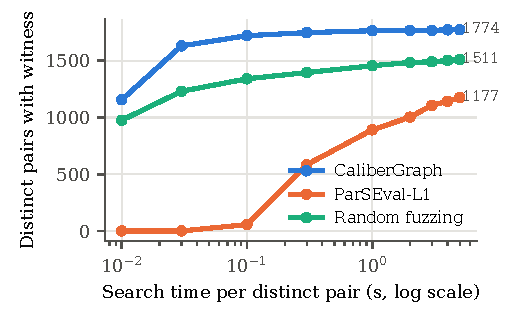
\includegraphics[width=0.75\linewidth]{figs/time_to_witness.pdf}
\caption{Distinct EX-correct pairs with a certified $\mathcal A_{1f}$ witness found within a given search time (first stage, 5\,s budget; a solver run that overruns the budget is not counted, so ParSEval-L1 reaches 1,177 of its 1,196 pairs).}\label{fig:time}
\end{figure}

In the first stage (Table~\ref{tab:ablation}), join-graph completion is the only component whose removal lowers the count significantly (\V{hFourNoJoinFullOnly} of \V{subFull} pairs lost, none gained; Holm-adjusted $p=0.004$); removing anchoring, isolation or the SQLite value domain changes the count by at most two pairs, and the median time to a witness stays at 6--8\,ms. \textbf{H4 is not supported}: the differences these components target are also reached by the other phases and by the mutation loop, which applies the same operators at random, so their benefit on development pairs did not carry over. In the second stage, the real sub-database phase accounts for most witnesses (\V{ablRNoReal} without it, $p=\V{ablRNoRealP}$, fewer than fuzzing-R), and anchored retrieval ($p=\V{ablRNoAnchorP}$) and join completion ($p=\V{ablRNoJoinP}$) also contribute, whereas constrained synthesis adds few witnesses ($p=\V{ablRNoSynP}$).

\textbf{Cost.} When CaliberGraph finds an $\mathcal A_{1f}$ witness, the median search time is \V{tCGMedian}\,s (\V{tCGWithinOne}\,\% within 1\,s; Fig.~\ref{fig:time}); ParSEval-L1 needs \V{tPVMedian}\,s and CaliberGraph-R \V{tCGRRMedian}\,s at $\mathcal A_R$, including its queries to $D_0$. Most distinct pairs, however, end without a witness after the full budget, so the budget dominates the cost: auditing the accepted test predictions of one system (about 800) alone with CaliberGraph-R takes \V{costSysMean} core-hours on average (\V{costSysMin}--\V{costSysMax}), or 6.9 core-hours for all ten systems when identical predictions are shared. Doubling the budget leaves CaliberGraph's count unchanged and raises ParSEval-L1's from \V{subPVFive} to \V{subPVTen}; at $\mathcal A_R$ (post hoc, same subsample) it changes CaliberGraph-R's count from 195 to 193 and fuzzing-R's from 151 to 153, so neither stage is budget-bound. Mining the profile is a one-time cost per benchmark (Section~\ref{sec:profile}). Attribution, which F2 (Table~\ref{tab:findings}) makes necessary, is a manual or model-assisted cost of a sample per tool and is not included.

\textbf{Root causes and benchmark issues.} In a sample of 100 first-stage CaliberGraph witnesses, AI-annotated in two passes (Table~\ref{tab:taxonomy} in the appendix), \texttt{NULL} handling (30\,\%), filter predicates (18\,\%) and join paths (17\,\%) cause two thirds of the differences, followed by ordering and \texttt{LIMIT} ties (12\,\%), duplicates (9\,\%) and aggregates over empty input (8\,\%). Across all attribution samples (77 items from schema-tier samples, 46 from $\mathcal A_R$ samples), \V{nIssues} distinct test questions received a witness that the AI annotators judged to expose a gold-query defect (\V{nIssuesGold}) or an ambiguous question (\V{nIssuesAmb}). \V{nIssuesFragile} of them are fragile: their witness lacks the entity the question names, or the two results differ only in rounding or letter case; the remaining \V{nIssuesRobust} comprise \V{nIssuesRobustGold} gold defects and \V{nIssuesRobustAmb} ambiguities. The gold defects are \emph{latent}: on $D_0$ the gold query returns the accepted answer, but on the witness it answers the question wrongly. Recurrent kinds are wrong join paths or attributes (11), filters that contradict the question's evidence (8: inclusive \texttt{BETWEEN} for strict bounds, equality for \texttt{LIKE}, case-sensitive matches), aggregates over an empty selection that return \texttt{NULL} where a count of zero is meant (7), counts of rows or names where entities are counted (7), and averages that count \texttt{NULL}s (3); about half of the ambiguities concern ties. We release the list, with one witness, the annotators' reasons and these flags per question, as a candidate list for maintainers rather than a verdict. The list overlaps only weakly with the corrected annotations of Jin et al.~\cite{jin2026annotation} (pre-registered): of the \V{arcG} questions we flag as gold defects that their Arcwise-Plat set covers, \V{arcGk} (\V{arcGpct}\,\%) received a gold query with a different result on $D_0$, against \V{arcNpct}\,\% of the \V{arcNN} unflagged test questions (one-sided Fisher $p=\V{arcPone}$); our ambiguity flags do not predict their edits (\V{arcApct}\,\% vs.\ \V{arcANpct}\,\%). Counting textual corrections of the gold query, which our witnesses can expose although the corrected query returns the same result on $D_0$, the rate is \V{arcGtextPct}\,\% against \V{arcNtextPct}\,\% (post hoc). \V{arcGuntouched} flagged gold defects and \V{arcAuntouched} flagged ambiguities were left entirely unchanged by Arcwise-Plat.


\subsection{RQ6: Replication on Spider and on new systems (Stage 3)}\label{sec:replication}
We re-ran the frozen code on Spider~1.0 dev~\cite{yu2018spider}, which no design decision had seen: 20 databases (\V{spTables} tables, \V{spRows}\,k rows), 1,034 questions and six public prediction sets (DAIL-SQL~\cite{gao2024dailsql} with and without self-consistency, Graphix-T5~\cite{li2023graphix}, DIN-SQL~\cite{pourreza2023dinsql}, GPT-4 few- and zero-shot), i.e., \V{spN} EX-correct pairs (117 pairs whose gold query fails on the Spider database are excluded). The pattern of the tiers replicates: CaliberGraph certifies \V{spCG} pairs at $\mathcal A_{1f}$ but \V{spCGR} at $\mathcal A_R$, fuzzing \V{spFZ} and \V{spFZR}. The search does not: CaliberGraph-R and fuzzing-R certify \V{spRCG} and \V{spRFZ} pairs at $\mathcal A_R$ (\V{spSOneA} vs.\ \V{spSOneB} discordant; one-sided $p=\V{spSOneP}$, CI over questions \V{spSOneLo} to \V{spSOneHi}; pre-registered S1 not supported), with equal recall on known positives (\V{spRecCGR} vs.\ \V{spRecFZR}\,\%). The attribution (two passes, $\kappa=\V{spKappa}$) finds \V{spImpCG} of \V{spNCG} sampled CaliberGraph witnesses implausible at $\mathcal A_{1f}$ against \V{spImpCGR} of \V{spNCGR} CaliberGraph-R witnesses at $\mathcal A_R$ (one-sided Fisher $p=\V{spSTwoP}$, not significant after Holm correction over the Stage-3 family) and none of \V{spNFZR} fuzzing-R witnesses; the estimated meaningful $\mathcal A_R$ witnesses are \V{spEstCGR} for CaliberGraph-R and \V{spEstFZR} for fuzzing-R (pre-registered S3 reversed: the difference has CI \V{spSThreeLo} to \V{spSThreeHi}, in fuzzing-R's favour). Post hoc, the implausible CaliberGraph-R witnesses almost all duplicate a real entity under a fresh key (two identical teachers), which the Spider profile does not forbid: on small tables our miner keeps only \V{spUcc} unique column combinations (BIRD: \V{bdUcc}), and \V{spCatShare}\,\% of the columns are categorical (BIRD: \V{bdCatShare}\,\%), so every admissible witness is close to a real sub-database and random real rows suffice.

On BIRD, the result of the search does replicate on systems the study had not seen: for the thirteen public prediction sets of BIRD Mini-Dev (GPT-3.5/4/4o, Llama-3, Mixtral, Phi-3), mapped to BIRD questions by the released question order (every mapped database matched, and the string literals of 88--93\,\% of predictions occur in the mapped question, evidence or gold query, against at most 15\,\% at neighbouring positions), restricted to held-out test questions and to (question, prediction) pairs not seen before, CaliberGraph-R certifies \V{mdCGR} of \V{mdN} new EX-correct pairs at $\mathcal A_R$ and fuzzing-R \V{mdFZR} (\V{mdA} vs.\ \V{mdB} discordant; CI over questions \V{mdLo}--\V{mdHi}; Holm-adjusted $p$ \V{holmEOne}). Of \V{mdAttrN} sampled CaliberGraph-R witnesses, \V{mdImp} were attributed to implausible data, close to the second-stage share (\V{pCGRImpl}\,\%), and \V{mdErr} to a prediction error.


\section{Lessons and Threats to Validity}\label{sec:threats}

% ICDE: summary of findings and recommendations
{\footnotesize
\begin{xltabular}{\textwidth}{@{}l >{\raggedright\arraybackslash}X >{\raggedright\arraybackslash}p{0.27\textwidth} >{\raggedright\arraybackslash}p{0.13\textwidth}@{}}
\caption{Summary of findings and recommendations.}\label{tab:findings}\\
\toprule
& Finding (evidence) & Recommendation & Audience\\
\midrule
\endfirsthead
\multicolumn{4}{@{}l}{\emph{Table~\ref{tab:findings}, continued}}\\
\toprule
& Finding (evidence) & Recommendation & Audience\\
\midrule
\endhead
\bottomrule
\endfoot
F1 & Under one SQLite certifier, released counterexamples lose about half of their pairs at the DDL tier and 82--92\,\% at the format tier. SpotIt, re-run under our budget, certifies \V{srLonef} pairs at $\mathcal A_{1f}$, against CaliberGraph's \V{nCGLonef}. The ranking of tools changes with the tier (Sec.~\ref{sec:main}). & Compare disprovers only under one certifier, tier and budget. Re-certify released witnesses on the benchmark's engine. & tool authors\\\addlinespace
F2 & By an LLM attribution, \V{attrImplMin}--\V{attrImplMax}\,\% of every tool's schema-tier witnesses rely on implausible data. Two humans shown facts of the data agreed (\V{hvTwoImpConsOne}/\V{hvTwoConsOne}). However, three further humans agreed with each other barely above chance (Fleiss' $\kappa_2=\V{hvThreeFleissBin}$), and their majority called \V{hvThreeImpOne}/\V{hvThreeMajOne} implausible. Humans attribute more witnesses to prediction errors than the AI does. A repair test removes \V{xVanPct}\,\% of the differences (Sec.~\ref{sec:validity}). & Report witnesses with an attributed sample, the data facts the judgment rests on and the annotators' agreement. Never report bare \emph{non-equivalent} counts. & tool authors, maintainers\\\addlinespace
F3 & A data profile of the benchmark takes minutes to mine. It cuts implausible witnesses from \V{pCGImpl}\,\% to \V{pCGRImpl}\,\% by the AI attribution; the human majority rates \V{hvThreeImpOne}/\V{hvThreeMajOne} vs.\ \V{hvThreeImpTwo}/\V{hvThreeMajTwo} as implausible. SpotIt+'s counterexamples (LLM-validated column constraints) are \V{pSIPImpl}\,\% implausible. Re-certified counts are insensitive to the profile's thresholds (Sec.~\ref{sec:rresults}). & Publish the data profile with the benchmark. Judge witnesses at $\mathcal A_R$, with a presupposition constraint for entities named in the question. & maintainers\\\addlinespace
F4 & At $\mathcal A_R$, counting witnesses lowers EX by \V{ptsCountRMin}--\V{ptsCountRMax} points per system, against 15--20 at $\mathcal A_{1f}$. Weighting by attributed error rates gives \V{ptsErrRMin}--\V{ptsErrRMax} points with the AI labels or \V{ptsHumThreeRMin}--\V{ptsHumThreeRMax} with the round-3 human majority (Sec.~\ref{sec:rankings}). & Never subtract witness counts from EX. Use meaningful witnesses to repair gold queries and questions. & maintainers, system builders\\\addlinespace
F5 & Join-graph completion and real-row retrieval matter, but three synthetic components do not. A data-grounded audit of one system's accepted test predictions costs under one core-hour at 5\,s per pair, plus attribution (Sec.~\ref{sec:ablation}). & Build disprovers on the join graph and real data. Certify and attribute every leaderboard submission. & tool authors, maintainers\\\addlinespace
F6 & On Spider, schema-tier witnesses again fail the profile, but CaliberGraph-R's lead does not replicate and fuzzing-R's witnesses are more meaningful. On 13 unseen BIRD systems, the lead in counts replicates (Sec.~\ref{sec:replication}). & Mine profiles from instances large enough to expose keys and dependencies, or add them by hand. & maintainers, tool authors\\
\end{xltabular}
}

\textbf{Lessons.} Table~\ref{tab:findings} maps each finding to a recommendation. The common thread is that a counterexample is a database and should be judged as data: certified on the benchmark's engine with the original query strings, checked against the benchmark's own profile, and released so that others can attribute it. Meaningful witnesses are feedback on the benchmark as well as on the systems. By the AI attribution, 58--64\,\% of the sampled data-grounded witnesses expose latent gold-query defects or ambiguous questions, against 11--22\,\% that expose prediction errors. Human annotators see more prediction errors (\V{humThreeErrPctR}\,\% by the round-3 majority), but they agree too little with each other for a reliable estimate. No correction of system scores can fix gold defects.

\textbf{Disproving is not proving.} A missing witness says nothing. Let \emph{semantic accuracy} at tier $\mathcal A$ be the share of predictions that are equivalent to the gold query under $(\mathcal C,\mathcal A)$. Accuracy corrected with witnesses at $\mathcal A$ is an upper bound on it, since every removed prediction is certified non-equivalent, while predictions with undetected differences remain counted. It is not a bound on the share of predictions that answer the question correctly, because witnesses that expose gold defects or ambiguities also remove predictions that may be right. Error-weighted corrections are lower bounds on the overstatement if the labels are unbiased. Bounded verifiers can also report the absence of counterexamples up to a bound, which our tools cannot do.

\textbf{What \emph{implausible} means.} The profile is mined from one instance, so it can be both too strict and too weak. It is too strict because a plausible but unobserved value is admitted only through range and shape rules. It is too weak because annotators still found conditional constraints that it does not express, such as a badge awarded once while others repeat; conditional-dependency and denial-constraint discovery could capture such constraints~\cite{fan2011cfd,chu2013dc}. \emph{Implausible} combines absence from the instance with a judgment about the domain, and annotators disagree on this judgment (Section~\ref{sec:validity}). A live football database may well contain unplayed fixtures without scores (Fig.~\ref{fig:example}). Conversely, a prediction that is right only because a column happens to hold no \texttt{NULL} is fragile under updates. An implausible witness therefore says that the benchmark, not the domain, cannot separate the queries. The same definition makes H7 close to circular: a judge who can query $D_0$ will rarely call a witness built from real rows of $D_0$ implausible. H7 thus checks that $\mathcal A_R$ works as constructed. The evidence that does not depend on the judge comes from mechanical outcomes: profile violations and repair survival (Section~\ref{sec:rresults}). Sub-databases can also omit the entity a question names (Section~\ref{sec:rresults}). Some differences rely on behavior that SQL leaves unspecified, such as which tied row \texttt{LIMIT} keeps. Because BIRD's EX is computed with SQLite, we count them, and attribution classifies most of them as ambiguities.

\textbf{AI-performed annotation.} All attribution and root-cause labels were produced by the AI model that also implemented the tools, in two independent passes plus adjudication. Agreement between the passes measures consistency, not correctness. The first author's earlier checks of two samples of 30 witnesses (agreement 26--28 of 30) were not blind: the AI verdicts were printed on the same sheet. A second model reproduces the labels (Section~\ref{sec:validity}), but both models share a vendor and the same data access. The human annotators of rounds 1--2, two data analysts familiar with SQL who volunteered, labeled independently. The pre-registered blind check failed in its first round, in which they had no access to $D_0$. In a second, separately pre-registered round with facts from $D_0$, they agreed with each other and reproduced the difference between the tiers, but they agreed with the AI only moderately. The two round-2 sheets contained a few manual edits outside the label fields: end-of-file markers, two altered witness cells in one item and a shortened fact line in another. The authors first attributed these edits to an editing tool. Excluding the two items changes no outcome. In round~3, three further unpaid analysts agreed barely above chance, and the process record of this round has the inconsistencies listed in Section~\ref{sec:validity}. The authors state that all three rounds were annotated by hand, and the round-3 annotators reported working without AI tools. All sheets are released as received, and the AI's estimated shares carry this uncertainty. Blinding to the tier is imperfect, since synthetic values such as \texttt{\textquotesingle{}x1\textquotesingle{}} and \texttt{-1} are recognizable. All annotations, reasons, witnesses and all human sheets are released.

\textbf{Baselines.} SpotIt was re-run from its released code under our budget (Section~\ref{sec:main}). Its bounded solver often exhausts five seconds, so a larger budget would favor it. Its released claims, obtained with larger budgets, are reported as well. SpotIt+ is used through its released outputs, since its constraint mining needs an LLM API that is unavailable in our environment. ParSEval-R certifies nothing at $\mathcal A_R$ and is not a fair representative of symbolic generation there. Unlike every other tool, the frozen first-stage fuzzing baseline accepted the first differing database without consulting the certifier. We re-ran exactly the affected pairs (132 distinct EX-correct, 259 EX-incorrect) with certifier-in-the-loop acceptance and the same seeds, and we report the corrected counts. The attribution sample of this baseline was drawn before the correction.

\textbf{Deviations from the pre-registrations.} The six documented deviations include adding the first-stage attribution after the first test run, adding the repair test post hoc, revising the data-profile tier on development data before the second freeze, and designing the second stage after seeing first-stage test attributions. Appendix~\ref{app:deviations} lists all deviations, and the artifact repository lists every amendment with its timestamp.

\textbf{Generalization.} All results concern SQLite, BIRD and Spider~1.0. The systems answer the same questions, and our intervals account for this by resampling questions. The tier was conceived after first-stage test attributions had been seen. Its only test on databases that no design decision had seen, Spider, did not replicate CaliberGraph-R's lead; the lead replicated only on new systems over the BIRD databases. Spider also shows that a profile mined from small instances is less informative. Larger enterprise schemas and other engines remain to be studied.

\section{Related Work}\label{sec:related}

\textbf{Execution-based Text-to-SQL evaluation.} Spider~\cite{yu2018spider} and BIRD~\cite{li2023bird} compare the results of the prediction and the gold query on one database. Test-suite accuracy~\cite{zhong2020testsuite} adds databases fuzzed around the original data and distilled to kill mutants of the gold query. The suite is fixed per gold query rather than targeted at a prediction. SQLMorph~\cite{malekpour2026sqlmorph} expands benchmark queries by mutation and replaces binary EX with fine-grained metrics. NL2SQL360~\cite{li2024nl2sql360} evaluates systems along many dimensions on fixed databases. FusionSQL~\cite{pham2026fusionsql} estimates accuracy without labels, and CycleSQL~\cite{fan2025cyclesql} validates translations through data provenance. These works change \emph{what} is measured on the benchmark data; we examine the \emph{evidence} that claimed EX false positives rest on. LLM judges such as FLEX~\cite{kim2025flex} and confidence estimators~\cite{somov2025confidence,maleki2026confidence} flag likely errors without checkable evidence. They can prioritize which predictions to audit. Studies of annotation noise in BIRD and Spider~\cite{wretblad2024noise,jin2026annotation} judge which query is intended. Jin et al.~\cite{jin2026annotation} release corrected annotations, against which we cross-check our issue list (Section~\ref{sec:ablation}). NL2SQLBench~\cite{hou2026nl2sqlbench} also reports inaccurate gold queries and overly strict comparison rules. Our witnesses attach a replayable database to each disagreement and surface such issues as a by-product. Alrashed et al.~\cite{alrashed2026verification} benchmark verifiers that accept or reject generated queries, including checks of execution consistency on synthetic data, and recommend defining correctness over several databases per question. Such checks presuppose that the databases are admissible, which is what our tiers quantify.

\textbf{Verification-based evaluation.} SpotIt~\cite{klopfenstein2026spotit} applies bounded equivalence verification, extended from VeriEQL~\cite{he2024verieql}, to search for distinguishing databases for BIRD predictions. SpotIt+~\cite{tremante2026spotitplus} adds constraints mined from the benchmark databases and validated by an LLM. Bounded verification can additionally show the absence of counterexamples up to a bound, but its coverage is limited by the encoded SQL fragment and semantics. We use both as the strongest baselines, re-run SpotIt from its released code under our budget, and re-certify all their counterexamples on SQLite.

\textbf{SQL equivalence.} Provers such as Cosette~\cite{chu2017cosette}, SQLSolver~\cite{ding2023sqlsolver} and QED~\cite{wang2024qed} establish equivalence for supported fragments. VeriEQL~\cite{he2024verieql} and Polygon~\cite{zhao2025polygon} search for bounded counterexamples. Classic results characterize containment of conjunctive and aggregate queries under set and bag semantics~\cite{chandra1977conjunctive,chaudhuri1993real,cohen2007aggregate}, and recent work bounds the number of rows needed to separate queries~\cite{cohen2026fewrows}. Under integrity constraints, equivalence and containment are decided with the chase for functional and inclusion dependencies~\cite{aho1979tableaux,johnson1984containment}. Our tiers play the role of such constraints for counterexample search, but they are mined from the instance rather than declared. These tools reason in a formal model. In contrast, we decide whether an admissible SQLite database separates two concrete query strings in the full dialect that LLMs produce, which includes string and date functions, \texttt{IIF}, \texttt{CAST}, window functions and type affinity.

\textbf{Query-aware test database generation.} QAGen~\cite{binnig2007qagen} and reverse query processing~\cite{binnig2007rqp} generate databases that make a query produce prescribed results. XData~\cite{chandra2015xdata} kills mutants of a correct query to grade student SQL. EvoSQL~\cite{castelein2018evosql} covers SQL predicates by search. ParSEval~\cite{chen2025parseval,chen2026parsevaldemo} performs plan-aware symbolic generation with a \texttt{disprove} mode for query pairs. These tools target coverage of one query or of a mutant space. CaliberGraph instead anchors the search on the actual differences between two queries and accepts only certified databases. ParSEval's interactive successor~\cite{chen2026parsevaldemo} lets users configure integrity assumptions (set or bag semantics, key and foreign-key constraints) and inspect witness databases. This overlaps with our tiers $\mathcal A_0$--$\mathcal A_1$. Our tier $\mathcal A_R$ adds constraints discovered from the benchmark instance, which are checked by a certifier independent of the generator. Constraint-driven generators such as DataSynth~\cite{arasu2011datasynth}, Touchstone~\cite{li2018touchstone} and SAM~\cite{yang2022sam} synthesize realistic databases for performance testing, not tiny databases that separate two queries.

\textbf{Real data for testing and data profiling.} Closest to CaliberGraph-R is RATest~\cite{miao2019ratest}, which explains why a query is wrong by finding a smallest sub-instance of a given test database on which it and a reference query return different results. RATest starts from a database that already separates the two queries and minimizes it for a human reader. For an EX-correct pair, $D_0$ does not separate the queries, so CaliberGraph-R must first find a real sub-database on which they differ. It accepts a candidate only if an independent certifier admits it under the data profile $\Pi$, which adds observed domains, undeclared inclusion dependencies and value dependencies to the declared constraints. We have not compared CaliberGraph-R with RATest or with another minimal-sub-instance baseline experimentally. Database subsetting tools such as Jailer~\cite{jailer} extract referentially intact subsets of production databases as test data, and Tuya et al.~\cite{tuya2016reduction} reduce a production database to a subset that preserves query coverage. In both, all rows are real, but neither targets the difference between two given queries. Data profiling discovers unique column combinations, inclusion dependencies and functional dependencies from an instance~\cite{abedjan2015profiling,papenbrock2016hyfd,papenbrock2015binder}. Our profile uses simple exhaustive queries, which suffice for BIRD's 3.9\,M rows; at larger scale, it could use these algorithms. Profiling features also drive error detection in data cleaning, e.g., ZeroED~\cite{ni2025zeroed}. We use these ideas in a new role: profiles of the benchmark database define the admissibility tier $\mathcal A_R$, and CaliberGraph-R searches real sub-databases that separate two given queries.

\section{Conclusion}\label{sec:conclusion}
A database on which a prediction and the gold query disagree is easy to misread. Under one certifier and budget, our disprover finds such databases for more accepted BIRD predictions than existing verifiers and test generators at DDL- and format-derived tiers, yet almost none of these witnesses satisfies a profile of the benchmark data, and judging whether they are evidence is hard: an AI annotator and two humans shown facts of the data rejected most of them, but three further humans agreed with each other barely above chance. Searching real sub-databases first certifies more profile-tier witnesses than random fuzzing on BIRD and on unseen systems, but not on Spider's small instances. At the profile tier, witnesses lower EX by about one to four points per system if weighted by attributed error rates and ten to thirteen if all are counted. We recommend that benchmarks publish their data profile and that audits report certified witnesses with the data facts they rest on and with the agreement of their annotators. Future work should add conditional and presupposition constraints to the profile, cover other engines, and develop attribution protocols that humans can reproduce.
\label{endconclusion}


\section*{Data and code availability}
All code, data, raw outputs, witness databases with certifier reports, AI and human annotations (every sheet as returned, with its key), the pre-registrations with their amendment log and freeze hashes, and the scripts that regenerate every number, table and figure are publicly available at \artifacturl{} under the Apache License 2.0 for our code and generated data. Material derived from BIRD and Spider is shared under CC BY-SA 4.0; third-party predictions and tools are used under their licences, listed in \texttt{THIRD\_PARTY\_NOTICES.md}. The BIRD and Spider databases themselves and the SpotIt/VeriEQL code are not redistributed.

\section*{Declaration of generative AI and AI-assisted technologies in the manuscript preparation process}
During the preparation of this work the authors used Claude Opus~5.5 (Anthropic) to draft and edit the manuscript text. The use of AI models in the research itself (study design, implementation, experiments and annotation) is described in Section~\ref{sec:aiuse}. After using this tool, the authors reviewed and edited the content as needed and take full responsibility for the content of the published article.

\section*{CRediT authorship contribution statement}
\textbf{Hongsheng Wang:} Conceptualization, Methodology, Software, Validation, Formal analysis, Investigation, Resources, Data curation, Writing -- original draft, Writing -- review \& editing, Project administration. The software, the analyses and the original draft were produced with an AI model under the author's direction and responsibility, as described in Section~\ref{sec:aiuse}. \textbf{Dazhen Deng:} Supervision, Writing -- review \& editing.

\section*{Funding}
This research did not receive any specific grant from funding agencies in the public, commercial, or not-for-profit sectors.

\section*{Declaration of competing interest}
The authors declare that they have no known competing financial interests or personal relationships that could have appeared to influence the work reported in this paper.

\section*{Acknowledgements}
We thank the human annotators, who volunteered their time.

\appendix
\section{Comparison contracts and root causes}\label{app:contracts}

\begin{table}[h]
\centering\small
\caption{First-freeze $\mathcal A_{1f}$ witnesses under the three comparison contracts (EX-correct test pairs; SpotIt and SpotIt+: re-certified released counterexamples; random fuzzing: corrected counts). Every $\mathcal C_{\mathrm{set}}$ difference is also a $\mathcal C_{\mathrm{bag}}$ difference; $\mathcal C_{\mathrm{len}}$ additionally equates an empty result with one all-\texttt{NULL} row and compares numbers to nine significant digits.}\label{tab:contracts}
\Tab{contracts}
\end{table}

\begin{table}[h]
\centering\small
\caption{Primary root cause of the difference for a random sample of 100 distinct first-freeze CaliberGraph witnesses (AI annotation, two independent passes, $\kappa=\V{taxKappa}$; no human check of root causes was made). Rule-based labels derived from the query structure contained the annotated primary cause in \V{taxRulePrimary} of 100 cases but assigned many additional labels, so we report the annotated causes.}\label{tab:taxonomy}
\Tab{taxonomy}
\end{table}

Differences caused by \texttt{NULL} handling, by filters and by join paths account for about two thirds of the sampled witnesses; ordering and \texttt{LIMIT} ties, duplicates and aggregates over empty inputs for most of the rest. These are also the classes in which the AI attribution most often finds implausible data (\texttt{NULL} in always-filled fields, duplicated entities) or ambiguous questions (ties).


\bibliographystyle{elsarticle-num}
\bibliography{references_verified}
\end{document}
